%Document-Author: Bonato Paolo + Biggeri Mattia + Nicoletti Luca
%Document-Date: 2016/03/24
%Document-Description: Documento di Specifica tecnica del gruppo SWEeneyThreads 

\documentclass[a4paper]{article}
\usepackage[english, italian]{babel}
\usepackage[T1]{fontenc}
\usepackage[utf8]{inputenc}
\usepackage{url}
\usepackage{graphicx}
\usepackage[hidelinks]{hyperref}
\usepackage{booktabs}
\usepackage{eurosym}
\usepackage{tabularx}
\usepackage{pifont}
\usepackage[table]{xcolor}
\usepackage{float}
\usepackage[]{appendix}
\usepackage{ltxtable} 
\usepackage{geometry}
\geometry{margin=1in}
\usepackage{longtable}
\usepackage{multirow}

\graphicspath{{Immagini/}}

\newcolumntype{Y}{>{\centering\arraybackslash}X}
\newcolumntype{s}{>{\hsize=.21\hsize}X}
\newcolumntype{f}{>{\hsize=.37\hsize}X}
\newcolumntype{m}{>{\hsize=.42\hsize}X}
\newcolumntype{t}{>{\hsize=.1\hsize}X}
\newcolumntype{r}{>{\hsize=.3\hsize}X}
\newcolumntype{k}{>{\hsize=.4\hsize}X}

\renewcommand{\abstractname}{Tabella contenuti}

\begin{document}
	
	\begin{titlepage}
		% Defines a new command for the horizontal lines, change thickness here
		\newcommand{\HRule}{\rule{\linewidth}{0.5mm}} 
		\center  
		
		% HEADING SECTION
		\textsc{\LARGE SWEeneyThreads}\\[1.5cm] 
		\textsc{\Large Actorbase}\\[0.5cm] 
		\textsc{\large a NoSQL DB based on the Actor model}\\[0.5cm]
		
		
		% TITLE SECTION
		\HRule \\[0.4cm]
		{ \huge \bfseries Specifica Tecnica}\\[0.4cm] 
		\HRule \\[1.5cm]
		
		% AUTHOR SECTION
		\begin{minipage}{0.4\textwidth}
			\begin{flushleft} \large
				\emph{Redattori:}\\
				Bortolazzo Matteo \\
				Nicoletti Luca  \\
			\end{flushleft}
		\end{minipage}
		~
		\begin{minipage}{0.4\textwidth}
			\begin{flushright} \large
				\emph{Approvazione:} \\
                    Bonato Paolo\\
				\emph{Verifica:} \\
                    Padovan Tommaso\\
                    Tommasin Davide \\
				 
			\end{flushright}
		\end{minipage}
		
		%immagine
		\begin{figure}[H]
			\centering
			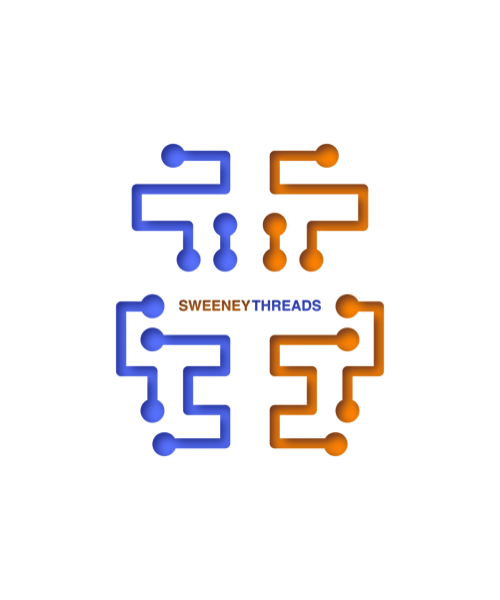
\includegraphics[scale=0.8]{sweeney.png}
		\end{figure}
		\begin{center}
			Versione 1.0.5
		\end{center}
		% Date, change the ->day to a set date if you want to be precise
		{\large \today} \\ [3cm] 
		% Fill the rest of the page with whitespace
		\vfill  
	\end{titlepage}
	
	
	\tableofcontents
	
	\newpage 
	\section*{Diario delle modifiche}
		\LTXtable{\textwidth}{Tabelle/tabelle_diario_modifiche/tabella_specifica.tex}

	\newpage \section{Introduzione}
	\subsection{Scopo del documento}
		Il documento illustra la progettazione attuale di Actorbase.
		Verranno presentati l'architettura, le componenti, le classi e i design pattern utilizzati.
	\subsection{Scopo del prodotto}
		Il progetto consiste nella realizzazione di un Database NoSQL key-value basato sul modello ad 
		Attori con l'obiettivo di fornire una tecnologia adatta allo sviluppo di moderne 
		applicazioni che richiedono brevissimi tempi di risposta e che elaborano enormi quantità 
		di dati. Lo sviluppo porterà al rilascio del software sotto licenza MIT.
	\subsection{Glossario}
		Al fine di evitare ambiguità di linguaggio e di massimizzare la comprensione dei documenti, il 
      gruppo ha steso un documento interno che è il \emph{Glossario v2.0.0}. In esso saranno definiti, in modo
      chiaro e conciso i termini che possono causare ambiguità o incomprensione del testo.
	\subsection{Riferimenti}
		\begin{itemize}
			\item \textbf{Slide dell'insegnamento Ingegneria del software mod.A:} \\
			\url{http://www.math.unipd.it/~tullio/IS-1/2015/Dispense/E02.pdf}
			\item \textbf{Scala:} \\
			\url{http://www.scala-lang.org/}
			\item \textbf{Java:} \\
			\url{http://www.java.com/}
			\item \textbf{Akka:} \\
			\url{http://akka.io/}
			\item \textbf{IntelliJ:} \\
			\url{http://www.jetbrains.com/idea/}
		\end{itemize}
	\subsubsection{Normativi}
		\begin{itemize}
			\item \textbf{Norme di progetto:} \emph{Norme di progetto v2.0.0}
			\item \textbf{Capitolato d'appalto Actorbase (C1):} \\ 
			\url{http://www.math.unipd.it/~tullio/IS-1/2015/Progetto/C1p.pdf}
		\end{itemize}
		
		
	\newpage 
	\section{Tecnologie utilizzate}
	\subsection{Scala}
		Le possibili scelte dettate dal capitolato sono Java e Scala. Si è scelto di utilizzare Scala perché offre i seguenti vantaggi:
		\begin{itemize}
            \item \textbf{Completamente Object-Oriented:} A differenza di Java, Scala è completamente orientato agli oggetti. Non c'è distinzione del tipo: oggetto - tipo primitivo, ogni valore è semplicemente un oggetto.
			\item \textbf{Staticamente tipato:} È un linguaggio tipato staticamente, questo permette di effettuare più facilmente i test. Inoltre Scala è in grado di stabilire il tipo di un oggetto per inferenza.
            \item \textbf{Può eseguire codice Java:} Scala può eseguire codice scritto in Java. È dunque possibile utilizzare classi e librerie scritte in Java all'interno di programmi scritti in Scala. 
            \item \textbf{Concorrenza e distribuzione:} Ottimo supporto alla programmazione multi-threaded e distribuita, essenziale per la realizzazione di un prodotto responsive e scalabile.
			\item \textbf{Supporto alla definizione di DSL:} Scala supporta nativamente la definizione di DSL.
            \item \textbf{Supporto di Akka:} Il linguaggio supporta la libreria Akka che è richiesta dal capitolato.
		\item \textbf{Preferenze del Committente:} Inoltre il Committente ha espresso esplicitamente la sua preferenza sull'utilizzo di Scala.
		\end{itemize}
		Problematiche di scala:
		\begin{itemize}
		\item \textbf{Familiarità con la tecnologia:} Nessun membro ha mai avuto esperienza, prima del inizio del progetto, con questo linguaggio di programmazione.
		\item \textbf{Leggibilità:} Alcuni costrutti risultano di difficile lettura.
		\end{itemize}
		\begin{figure} [H]
			\centering
			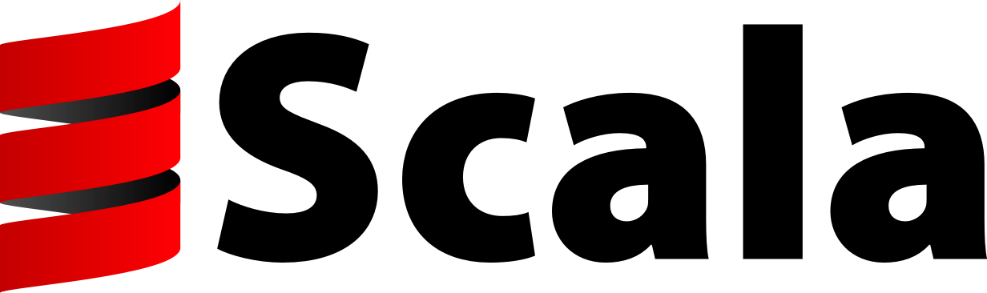
\includegraphics[scale=0.15]{immagini/ST/scala.png}
			\caption{Scala - logo}
		\end{figure}	
	\subsection{Akka}
		L'utilizzo della libreria Akka oltre ad essere reso obbligatorio dal committente, fornisce un'eccellente base su cui sviluppare un sistema basato sul modello ad attori.
        Akka permette di costruire facilmente applicazioni message-driven che siano estremamente concorrenti, distribuite e resilienti.         
        La natura distribuita e asincrona degli attori messi a disposizione da Akka soddisfa pienamente i bisogni del sistema da implementare.
        Akka esegue l'ovveride di molti operatori rendendo difficile la comprensione agli utenti poco esperti. 
	\begin{figure} [H]
			\centering
			
\includegraphics[width=\textwidth]{immagini/ST/Akka.png}
			\caption{Akka - logo}
		\end{figure}	
	
	
	\newpage 
	\section{Legenda}
	Tutti gli schemi dei package seguono la legenda sottostante. I livelli di annidamento sono da intendere per la totale struttura dei package e non solo per il singolo schema.
		\begin{figure} [H]
			\centering
			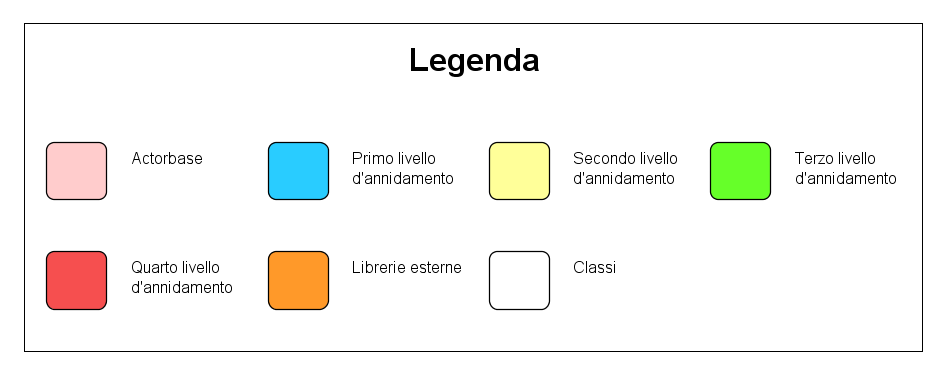
\includegraphics[scale=0.3]{ST/Legenda}
			\caption{Legenda}
		\end{figure}
		
	\section{Descrizione dell'architettura}
		\subsection{Metodo e formalismo di specifica}
			Nell'esposizione dell'architettura del prodotto si procederà con un approccio di tipo top-down. \\
			Inizialmente si descriveranno le tre componenti fondamentali: Client, Server e Driver; poi le componenti più piccole al loro interno, 
			specificando i package e le classi che li compongono. \\ \\
			Per ogni package saranno descritti brevemente il tipo, l'obiettivo e la funzione e saranno specificati eventuali figli, classi ed 
			interazioni con altri package. Ogni classe sarà dotata di una breve descrizione e ne saranno specificate le responsabilità, 
			le classi ereditate, le sottoclassi e le relazioni con altre classi. \\
			Successivamente saranno mostrati e descritti i diagrammi delle attività che coinvolgono l'utente. \\
			Infine si illustreranno degli esempi di utilizzo dei design pattern nell'architettura del sistema.
		\subsection{Architettura generale}
        	L'architettura generale del sistema è di tipo client-server. \\ \\
            Il Server ha un'architettura di tipo event-driven basata sul modello ad attori e accetta connessioni in entrata tramite un socket TCP. \\ \\
			Il Client è un semplice programma che espone un'interfaccia a linea di comando per accettare comandi che vengono inoltrati al Server tramite 
			il Driver.
            
        \begin{figure} [H]
			\centering
			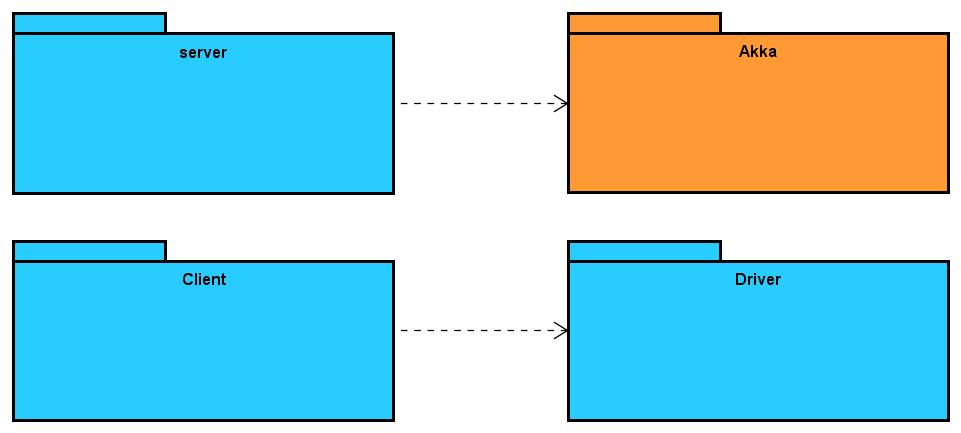
\includegraphics[width=\textwidth]{ST/generalLevel.jpg}
			\caption{Architettura generale, vista Package}
		\end{figure}
		
        \subsubsection{Server}
		
        	Il Server di \emph{Actorbase} è composto da quattro package principali ed una classe: 
			i package \textbf{utils}, \textbf{messages}, \textbf{actors} ed \textbf{enums} e la classe \textbf{Server}. \\
			
			Il package \textbf{utils} contiene delle classi di supporto che vengono utilizzate dai vari attori presenti per effettuare operazioni 
			di vario genere. \\
			Il package \textbf{messages} contiene tutte le interfacce e le classi dei messaggi che gli attori possono mandarsi tra di loro. \\
			Il package \textbf{actors} contiene tutte le classi che definisco gli attori del sistema. \\
			Il package \textbf{enums} contiene le enumerazioni utilizzate per vari scopi. \\
			\\
			\noindent La classe \textbf{Server} è l'entry point del programma e gestisce la configurazione iniziale all'avvio dello stesso.  
			            
		
        \subsubsection{Client}
		
        	Il Client di \emph{Actorbase} è composto da due sole classi: \textbf{Client} e \textbf{Welcome}, entrambe \emph{Singleton}.

        \subsubsection{Driver}
		
        	Il Driver è una libreria, invocando i metodi della quale è possibile effettuare richieste TCP sul socket su cui il
			Server è in ascolto. \\
			Contiene due classi e un'interfaccia: l'interfaccia \textbf{Connection}, le classi \textbf{Driver} e \textbf{ConcreteConnection}. 
			Quest'ultima è una realizzazione dell'interfaccia \textbf{Connection}. 

				
	\newpage 
	\section{Componenti e Classi}
	
		\subsection{Actorbase}
			
			\subsubsection{Descrizione}
				È il livello principale del sistema. L'interazione tra le componenti dei package \textbf{Server} e \textbf{Driver} avviene tramite una 
				connessione di rete TCP di tipo client-server.
				
			\subsubsection{Package Figli}
				\begin{itemize}
					\item Actorbase.server
					\item Actorbase.client
					\item Actorbase.driver
				\end{itemize}
				
		\subsection{Actorbase.server}
		
			\begin{figure}[H]
				\centering
				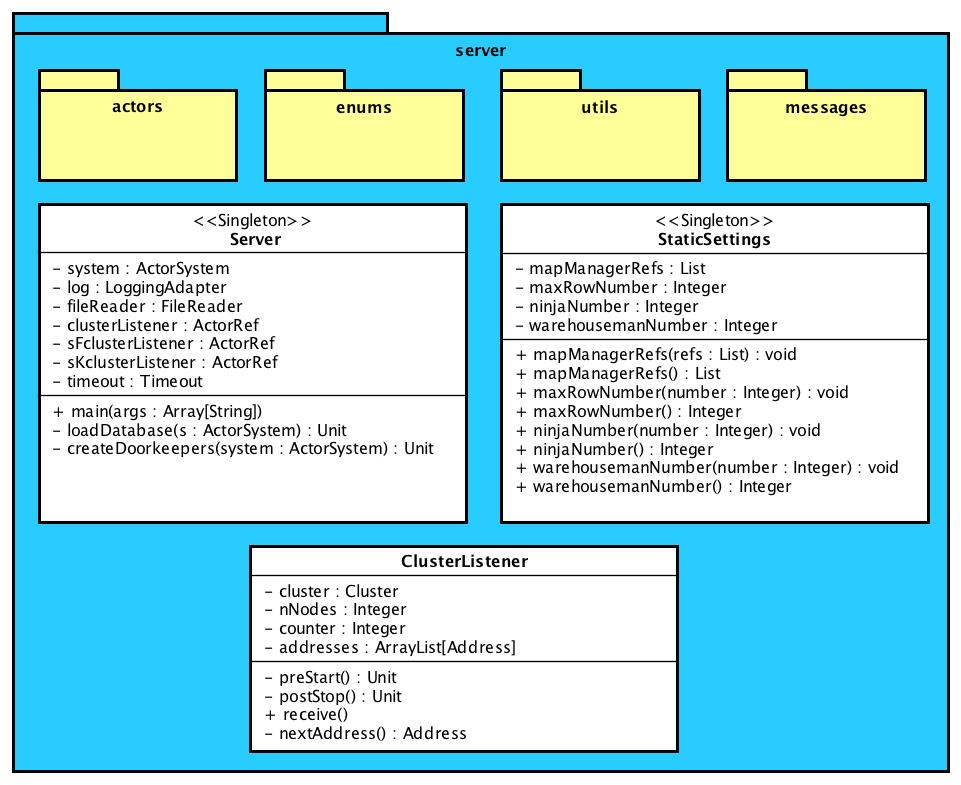
\includegraphics[width=\textwidth]{ST/Server/serverLevel.jpg}
				\caption{Componente Actorbase.server}
			\end{figure}
			\subsubsection{Descrizione}
				Package per la componente lato server del sistema. 
				È composto dai package \textbf{utils}, \textbf{messages}, \textbf{actors} ed \textbf{enums} e dalla classe \textbf{Server}.\\
				
			\subsubsection{Package Figli}
				\begin{itemize}
					\item Actorbase.server.utils
					\item Actorbase.server.messages
					\item Actorbase.server.actors
					\item Actorbase.server.enums
				\end{itemize}
				
			\subsubsection{Classi}
				\begin{itemize}
					\item Actorbase.server.Server
				\end{itemize}
				
		\subsection{Actorbase.server.Server}
			\subsubsection{Descrizione}
				Classe principale della parte \textbf{Server} del programma. È di fatto l'entry point dello stesso, gestisce la configurazione 
				iniziale e avvia il sistema. Utilizza il design pattern \textbf{Singleton}.
				
			\subsubsection{Utilizzo}
				Classe che fornisce un punto di accesso al programma, la sua esecuzione avvia il server sulla macchina in cui viene lanciata.
				
			\subsubsection{Relazione con altre classi}
				\begin{itemize}
					\item \textbf{Actorbase.server.actors.Doorkeeper:} relazione uscente, creazione.
					\item \textbf{Actorbase.server.actors.Main:} relazione di utilizzo.
					\item \textbf{Actorbase.server.utils.FileManager:} relazione uscente, creazione.
				\end{itemize}
				
		\subsection{Actorbase.server.utils}
		
			\begin{figure} [H]
				\centering
				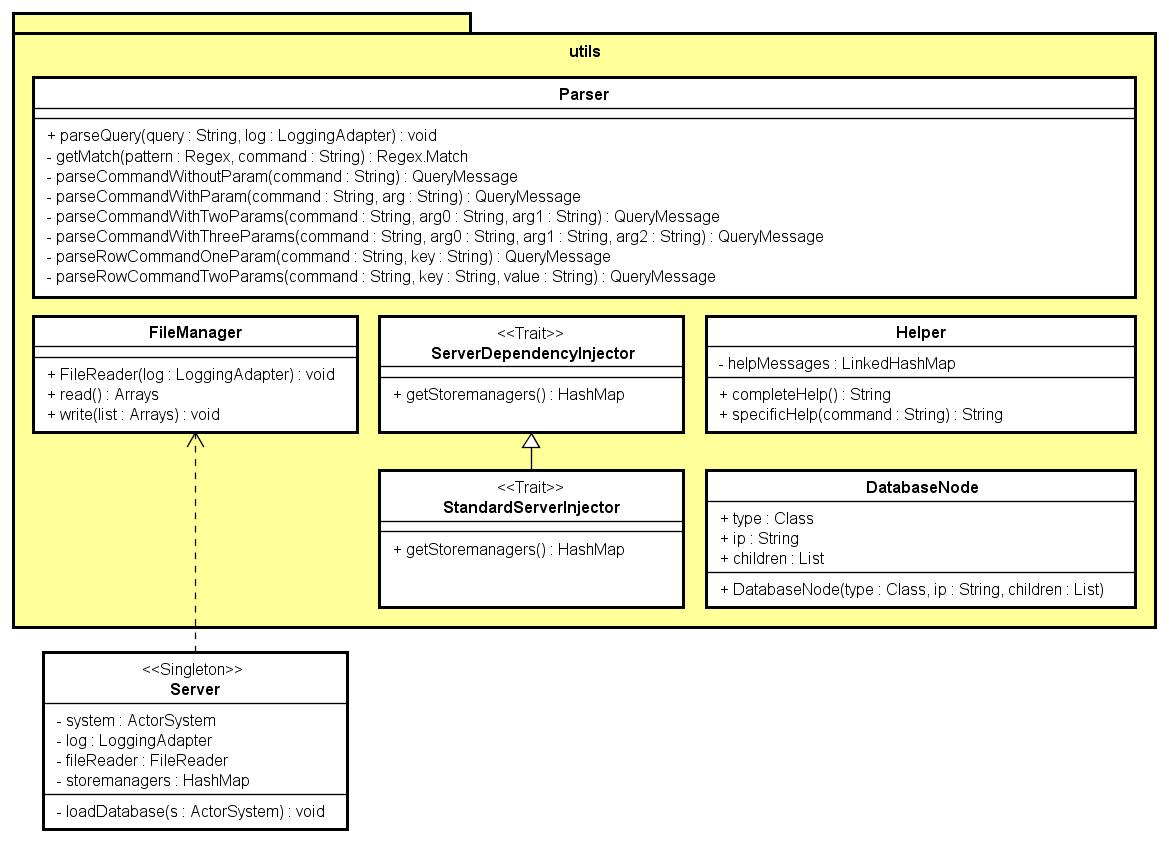
\includegraphics[width=\textwidth]{ST/Server/utilsLevel.jpg}
				\caption{Componente Actorbase.server.utils}
			\end{figure}
			
			\subsubsection{Descrizione}
				Package contenente le classi che effettuano operazioni varie a supporto delle varie componenti del server, e degli attori nello specifico.
				
			\subsubsection{Classi}
				\begin{itemize}
					\item Actorbase.server.utils.Parser
					\item Actorbase.server.utils.FileManager
					\item Actorbase.server.utils.Helper
					\item Actorbase.server.utils.DatabaseNode
				\end{itemize}
				
			\subsubsection{Trait}
				\begin{itemize}
					\item Actorbase.server.utils.ServerDependencyInjector
					\item Actorbase.server.utils.StandardServerInjector
				\end{itemize}
				
		\subsection{Actorbase.server.utils.ServerDependencyInjector}
			\subsubsection{Descrizione}
				Trait che espone i metodi necessari per le interrogazioni al server da parte del \textbf{Main}.
				
			\subsubsection{Utilizzo}
				Viene utilizzato per delegare la chiamata ai metodi del Server ad un'interfaccia in modo da poter utilizzare server differenti in base 
				alle necessità.
				
			\subsubsection{Relazione con altre classi}
				\begin{itemize}
					\item \textbf{Actorbase.server.actors.Main:} relazione entrante, aggregazione.
				\end{itemize}
				
			\subsubsection{Classi figlie}
				\begin{itemize}
					\item Actorbase.server.utils.StandardServerInjector
				\end{itemize}
		
		\subsection{Actorbase.server.utils.StandardServerInjector}
			\subsubsection{Descrizione}
				Implementazione del trait \textbf{ServerDependencyInjector} che utilizza il server da noi creato.
				
			\subsubsection{Utilizzo}
				Viene utilizzato per delegare la chiamata ai metodi del Server ad un'interfaccia in modo da poter utilizzare server differenti in base 
				alle necessità.				
				
			\subsubsection{Relazione con altre classi}
				\begin{itemize}
					\item \textbf{Actorbase.server.actors.Main:} relazione entrante, aggregazione.
				\end{itemize}
			
		\subsection{Actorbase.server.utils.Parser}
			\subsubsection{Descrizione}
				Classe utilizzata dal server per tradurre la stringa ricevuta da un client in un messaggio che ne rappresenta la richiesta per la 
				comunicazione tra attori.
				
			\subsubsection{Utilizzo}
				Viene utilizzata dal Server quando esso riceve una richiesta da un Client.
				
			\subsubsection{Relazione con altre classi}
			\begin{itemize}
				\item \textbf{Actorbase.server.actors.Usermanager:} relazione entrante, creazione.
				\item \textbf{Actorbase.server.messages.QueryMessages.QueryMessage:} relazione uscente, creazione. 
			\end{itemize}
		
		\subsection{Actorbase.server.utils.FileManager}
			\subsubsection{Descrizione}
				Classe utilizzata dagli attori per gestire i file su disco.
				
			\subsubsection{Utilizzo}
				Viene utilizzata dalla maggior parte degli attori quando necessitano di leggere o scrivere su file.
				
			\subsubsection{Relazione con altre classi}
				\begin{itemize}
					\item \textbf{Actorbase.server.Server:} relazione entrante, creazione.
					\item \textbf{Actorbase.server.actors.Warehouseman:} relazione entrante, creazione.
					\item \textbf{Actorbase.server.utils.DatabaseNode:} relazione uscente, creazione. 
				\end{itemize}
				
		\subsection{Actorbase.server.utils.Helper}
			\subsubsection{Descrizione}
				Classe che mette a disposizione dei metodi per visualizzare la lista di comandi disponibili e la loro spiegazione.
				
			\subsubsection{Utilizzo}
				Viene utilizzata dall'attore Main per recuperare la lista di comandi con la loro spiegazione, è anche possibile recuperare 
				la spiegazione di un singolo comando.
				
			\subsubsection{Relazione con altre classi}
				\begin{itemize}
					\item \textbf{Actorbase.server.actors.Main:} relazione entrante, creazione. 
				\end{itemize}
			
		\subsection{Actorbase.server.utils.DatabaseNode}
			\subsubsection{Descrizione}
				Classe utilizzata per costruire l'albero che rappresenta la struttura gerarchica delle componenti del database,
				è costituita da un singolo nodo e tutti i suoi discendenti.
				
			\subsubsection{Utilizzo}
				Viene utilizzata da tutti gli attori presenti nel database al momento della sua chiusura e apertura per salvare e ricostruire 
				la struttura gerarchica.
				
			\subsubsection{Relazione con altre classi}
				\begin{itemize}
					\item \textbf{Actorbase.server.Server:} relazione entrante, creazione.
					\item \textbf{Actorbase.server.actors.Main:} relazione entrante, creazione.
					\item \textbf{Actorbase.server.actors.Doorkeeper:} relazione entrante, creazione.
					\item \textbf{Actorbase.server.actors.Storefinder:} relazione entrante, creazione.
					\item \textbf{Actorbase.server.actors.Storekeeper:} relazione entrante, creazione.
					\item \textbf{Actorbase.server.actors.Warehouseman:} relazione entrante, creazione.
					\item \textbf{Actorbase.server.actors.Usermanager:} relazione entrante, creazione.
					\item \textbf{Actorbase.server.actors.Storemanager:} relazione entrante, creazione.
					\item \textbf{Actorbase.server.utils.FileManager:} relazione entrante, creazione.
				\end{itemize}
				
		\subsection{Actorbase.server.actors}
		
			\begin{figure} [H]
				\centering
				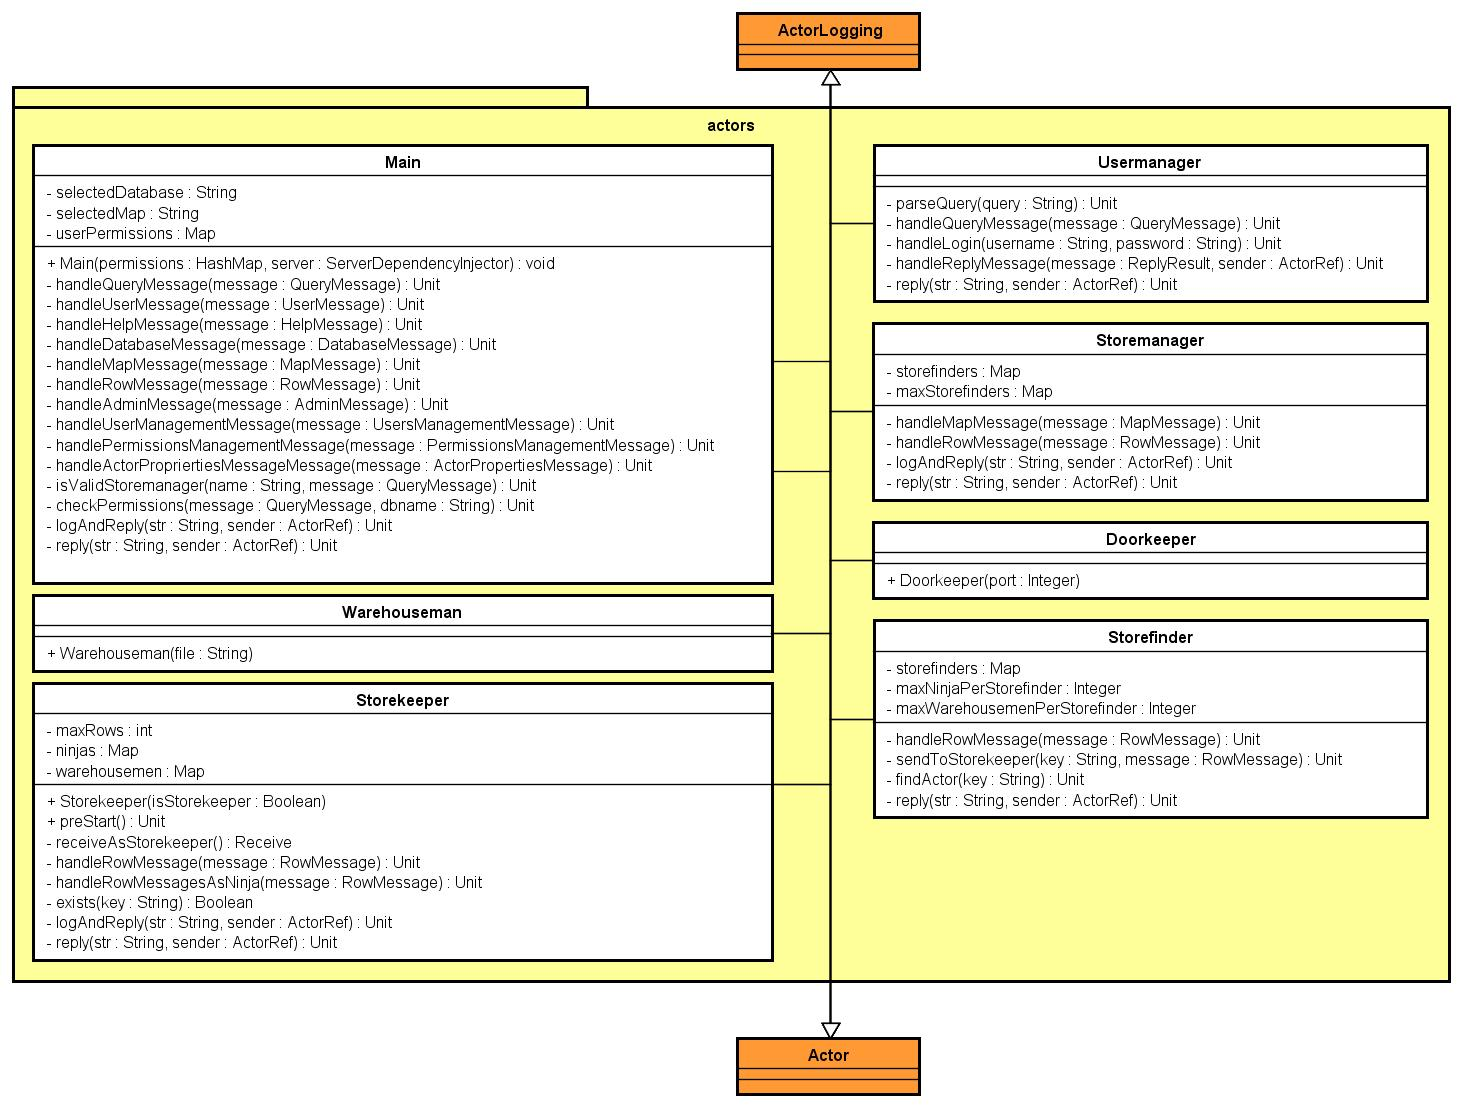
\includegraphics[width=\textwidth]{ST/Server/actorsLevel.jpg}
				\caption{Componente Actorbase.server.actors}
			\end{figure}
			
			\subsubsection{Descrizione}
				Package contenente tutti gli attori che compongono il database.
				
			\subsubsection{Classi}
				\begin{itemize}
					\item Actorbase.server.actors.Main
					\item Actorbase.server.actors.Doorkeeper
					\item Actorbase.server.actors.Storekeeper
					\item Actorbase.server.actors.Storefinder
					\item Actorbase.server.actors.Warehouseman
					\item Actorbase.server.actors.Usermanager
					\item Actorbase.server.actors.Storemanager
				\end{itemize}
		
		\subsection{Actorbase.server.actors.Doorkeeper}
			\subsubsection{Descrizione}
				Questo attore apre il socket su cui i client potranno connettersi, crea un attore \textbf{Usermanager} per ogni nuova 
				connessione ed inoltra ogni messaggio ricevuto dal client e  all'\textbf{Usermanager} ad esso associato.
				
			\subsubsection{Utilizzo}
				Viene utilizzato per aprire un socket e resta in attesa di richieste di connessione da parte di client.
				
			\subsubsection{Relazione con altre classi}
				\begin{itemize}
					\item \textbf{Actorbase.server.Server:} relazione entrante, creazione.
					\item \textbf{Actorbase.server.actors.Usermanager:} relazione uscente, creazione.
					\item \textbf{Actorbase.server.utils.ReplyResult:} relazione di utilizzo.
				\end{itemize}
				
		\subsection{Actorbase.server.actors.Usermanager}
			\subsubsection{Descrizione}
				Questo attore si preoccupa di trasformare le stringhe ricevute dal client in messaggi interpretabili da altri attori.
				
			\subsubsection{Utilizzo}
				Viene utilizzato per gestire una connessione da parte di un client, crea un attore \textbf{Main} e invia le richieste 
				ricevute all'attore creato. 
				
			\subsubsection{Relazione con altre classi}
				\begin{itemize}
					\item \textbf{Actorbase.server.actors.Doorkeeper:} relazione entrante, creazione.
					\item \textbf{Actorbase.server.actors.Main:} relazione uscente, creazione.
					\item \textbf{Actorbase.server.utils.Parser:} relazione uscente, creazione.
					\item \textbf{Actorbase.server.utils.ReplyResult:} relazione di utilizzo.
					\item \textbf{Actorbase.server.messages.query.QueryMessage:} relazione di utilizzo.
				\end{itemize}
				
		\subsection{Actorbase.server.actors.Main}
			\subsubsection{Descrizione}
				Questo attore è responsabile del controllo dei permessi delle richieste ricevute. Gestisce tutti i messaggi, elaborandoli o inoltrandoli 
				se non di sua competenza.
				
			\subsubsection{Utilizzo}
				Viene utilizzato per controllare i permessi delle richieste ricevute, gestisce i messaggi a livello di database e di help
				 e inoltra tutti gli altri messaggi che non sono di sua competenza. Inoltre si preoccupa di mantenere in memoria le selezioni di 
				 database e mappa effettuate dall'utente.
				
			\subsubsection{Relazione con altre classi}
				\begin{itemize}
					\item \textbf{Actorbase.server.Server:} relazione di utilizzo.
					\item \textbf{Actorbase.server.actors.Usermanager:} relazione entrante, creazione.
					\item \textbf{Actorbase.server.actors.Storemanager:} relazione di utilizzo.
					\item \textbf{Actorbase.server.actors.Storefinder:} relazione uscente, creazione.
					\item \textbf{Actorbase.server.utils.Helper:} relazione uscente, creazione.
					\item \textbf{Actorbase.server.Permission:} relazione di utilizzo.
					\item \textbf{Actorbase.server.utils.ReplyResult:} relazione di utilizzo.
					\item \textbf{Actorbase.server.messages.query.QueryMessage:} relazione di utilizzo.
					\item \textbf{Actorbase.server.messages.query.ReplyMessage:} relazione di utilizzo.
					\item \textbf{Actorbase.server.messages.query.PermissionMessages.NoPermissionMessage:} relazione di utilizzo.
					\item \textbf{Actorbase.server.messages.query.PermissionMessages.AdminPermissionMessage:} relazione di utilizzo.
					\item \textbf{Actorbase.server.messages.internal.AskMapMessage:} relazione uscente, creazione e utilizzo.
					\item \textbf{Actorbase.server.messages.internal.BecomeStorekeeperMessage:} relazione di utilizzo.
					\item \textbf{Actorbase.server.messages.internal.SendMapMessage:} relazione di utilizzo.
					\item \textbf{Actorbase.server.messages.internal.LinkMessages.LinkMessage:} relazione di utilizzo.
				\end{itemize}
				
		\subsection{Actorbase.server.actors.Storemanager}
			\subsubsection{Descrizione}
				Questo attore rappresenta un database o una sua parte.
				
			\subsubsection{Utilizzo}
				Viene utilizzato per gestire tutti i messaggi a livello mappa, e inoltra tutti gli altri messaggi che non sono di sua competenza.
				
			\subsubsection{Relazione con altre classi}
				\begin{itemize}
					\item \textbf{Actorbase.server.Server:} relazione entrante, creazione.
					\item \textbf{Actorbase.server.actors.Main:} relazione di utilizzo.
					\item \textbf{Actorbase.server.actors.Storefinder:} relazione uscente, creazione.
					\item \textbf{Actorbase.server.utils.ReplyResult:} relazione di utilizzo.
					\item \textbf{Actorbase.server.messages.query.user.UserMessage:} relazione di utilizzo.
				\end{itemize}
				
		\subsection{Actorbase.server.actors.Storefinder}
			\subsubsection{Descrizione}
				Questo attore rappresenta una mappa o una sua parte.
				
			\subsubsection{Utilizzo}
				Viene utilizzato per gestire gli \textbf{Storekeeper} a cui inoltra i messaggi.
				
			\subsubsection{Relazione con altre classi}
				\begin{itemize}
					\item \textbf{Actorbase.server.actors.Storemanager:} relazione entrante, creazione.
					\item \textbf{Actorbase.server.actors.Storekeeper:} relazione uscente, creazione.
					\item \textbf{Actorbase.server.actors.Warehouseman:} relazione uscente, creazione.
					\item \textbf{Actorbase.server.utils.ReplyResult:} relazione di utilizzo.
					\item \textbf{Actorbase.server.messages.query.users.RowMessages.RowMessage:} relazione di utilizzo.
					\item \textbf{Actorbase.server.message.internal.BecomeStorekeeperMessage:} relazione uscente, creazione e utilizzo.
					\item \textbf{Actorbase.server.messages.internal.LinkMessages.LinkMessage:} relazione uscente, creazione e utilizzo.
				\end{itemize}
				
		\subsection{Actorbase.server.actors.Storekeeper}
			\subsubsection{Descrizione}
				Questo attore contiene una parte di mappa. Esso ha anche funzionalità di backup, qualora uno \textbf{Storekeeper} morisse, 
				un altro potrebbe subentrare al suo posto.
				
			\subsubsection{Utilizzo}
				Viene utilizzato per memorizzare in memoria RAM le entry presenti in una mappa, gestisce i messaggi a livello di riga.
				Quando un attore della stessa classe a cui esso è associato si spegne, esso diventa la copia ufficiale della parte di mappa 
				da esso rappresentata.
				
			\subsubsection{Relazione con altre classi}
				\begin{itemize}
					\item \textbf{Actorbase.server.actors.Storefinder:} relazione entrante, creazione.
					\item \textbf{Actorbase.server.actors.Warehouseman:} relazione di utilizzo.
					\item \textbf{Actorbase.server.utils.ReplyResult:} relazione di utilizzo.
					\item \textbf{Actorbase.server.messages.query.users.RowMessages.RowMessage:} relazione di utilizzo.
					\item \textbf{Actorbase.server.message.internal.BecomeStorekeeperMessage:} relazione di utilizzo.
					\item \textbf{Actorbase.server.messages.internal.SendMapMessage:} relazione di utilizzo.
					\item \textbf{Actorbase.server.messages.internal.LinkMessages.LinkMessage:} relazione di utilizzo.
				\end{itemize}
		
		\subsection{Actorbase.server.actors.Warehouseman}
			\subsubsection{Descrizione}
				Questo attore permette l'interazione del database con il filesystem.
				
			\subsubsection{Utilizzo}
				Viene utilizzato per mantenere un backup del database su file presenti su disco. 
				
			\subsubsection{Relazione con altre classi}
				\begin{itemize}
					\item \textbf{Actorbase.server.actors.Storekeeper:} relazione di utilizzo.
					\item \textbf{Actorbase.server.actors.Storefinder:} relazione entrante, creazione.
					\item \textbf{Actorbase.server.utils.ReplyResult:} relazione di utilizzo.
					\item \textbf{Actorbase.server.messages.query.users.RowMessages.RowMessage:} relazione di utilizzo.
					\item \textbf{Actorbase.server.messages.internal.SendMapMessage:} relazione uscente, creazione e utilizzo.
				\end{itemize}
				
		\subsection{Actorbase.server.enums}
		
			\begin{figure} [H]
				\centering
				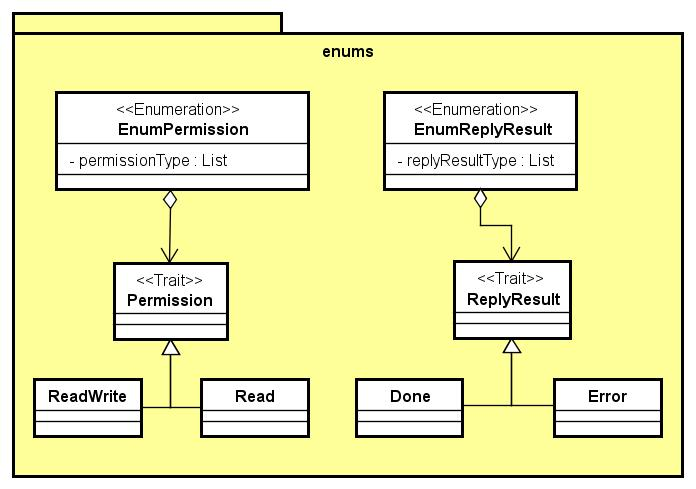
\includegraphics[width=\textwidth]{ST/Server/enumsLevel.jpg}
				\caption{Componente Actorbase.server.enums}
			\end{figure}
			
			\subsubsection{Descrizione}
				Package contenente le enumerazioni utilizzate dagli attori per distinguere i tipi di permessi e di risposte.
				
			\subsubsection{Classi}
				\begin{itemize}
					\item Actorbase.server.enums.Read
					\item Actorbase.server.enums.ReadWrite
					\item Actorbase.server.enums.Done
					\item Actorbase.server.enums.Error
					\item Actorbase.server.enums.EnumPermission
					\item Actorbase.server.enums.EnumReplyResult
				\end{itemize}
				
			\subsubsection{Trait}
				\begin{itemize}
					\item Actorbase.server.utils.Permission
					\item Actorbase.server.utils.ReplyResult
				\end{itemize}
		
		\subsection{Actorbase.server.enums.Permission}
			\subsubsection{Descrizione}
				Trait per rappresentare i permessi che la richiesta di un utente può avere.
				
			\subsubsection{Utilizzo}
				Viene utilizzata dall'attore \textbf{Main} per effettuare i controlli dei permessi dei messaggi. 				
				
			\subsubsection{Relazione con altre classi}
				\begin{itemize}
					\item \textbf{Actorbase.server.actors.Main:} relazione di utilizzo.
					\item \textbf{Actorbase.server.enums.EnumPermission:} relazione entrante, aggregazione.
				\end{itemize}
				
			\subsubsection{Classi figlie}
				\begin{itemize}
					\item Actorbase.server.enums.Read.
					\item Actorbase.server.enums.ReadWrite.
				\end{itemize}
				
		\subsection{Actorbase.server.enums.ReplyResult}
			\subsubsection{Descrizione}
				Trait per rappresentare le risposte ed il loro stato (avvenuta con successo, errore). 
				
			\subsubsection{Utilizzo}
				Viene utilizzata da tutti gli attori per indicare se la richiesta effettuata da un utente è andata a buon fine o no.
				
			\subsubsection{Relazione con altre classi}
				\begin{itemize}
					\item \textbf{Actorbase.server.actors.Main:} relazione di utilizzo.
					\item \textbf{Actorbase.server.actors.Doorkeeper:} relazione di utilizzo.
					\item \textbf{Actorbase.server.actors.Storefinder:} relazione di utilizzo.
					\item \textbf{Actorbase.server.actors.Storekeeper:} relazione di utilizzo.
					\item \textbf{Actorbase.server.actors.Warehouseman:} relazione di utilizzo.
					\item \textbf{Actorbase.server.actors.Usermanager:} relazione di utilizzo.
					\item \textbf{Actorbase.server.actors.Storemanager:} relazione di utilizzo.
					\item \textbf{Actorbase.server.enums.EnumReplyResult:} relazione entrante, aggregazione.
				\end{itemize}
				
			\subsubsection{Classi figlie}
				\begin{itemize}
					\item Actorbase.server.enums.Error.
					\item Actorbase.server.enums.Done.
				\end{itemize}				
						
		\subsection{Actorbase.server.enums.Read}
			\subsubsection{Descrizione}
				Questa classe rappresenta il permesso di lettura.
				
			\subsubsection{Utilizzo}
				Viene utilizzata dall'attore \textbf{Main} per effettuare i controlli dei permessi dei messaggi. 
				
			\subsubsection{Relazione con altre classi}
				\begin{itemize}
					\item \textbf{Actorbase.server.actors.Main:} relazione di utilizzo.
				\end{itemize}
						
			\subsubsection{Trait implementati}
				\begin{itemize}
					\item \textbf{Actorbase.server.enums.Permission} 
				\end{itemize}
				
		\subsection{Actorbase.server.enums.Write}
			\subsubsection{Descrizione}
				Questa classe rappresenta il permesso di scrittura.
				
			\subsubsection{Utilizzo}
				Viene utilizzata dall'attore \textbf{Main} per effettuare i controlli dei permessi dei messaggi. 
				
			\subsubsection{Relazione con altre classi}
				\begin{itemize}
					\item \textbf{Actorbase.server.actors.Main:} relazione di utilizzo.
				\end{itemize}
				
			\subsubsection{Trait implementati}
				\begin{itemize}
					\item \textbf{Actorbase.server.enums.Permission} 
				\end{itemize}
		
		\subsection{Actorbase.server.enums.Done}
			\subsubsection{Descrizione}
				Questa classe rappresenta l'avvenuto successo di una richiesta effettuata da un utente.
				
			\subsubsection{Utilizzo}
				Viene utilizzata da tutti gli attori come risposta in caso di richiesta effettuata con successo.
				
			\subsubsection{Relazione con altre classi}
				\begin{itemize}
					\item \textbf{Actorbase.server.actors.Main:} relazione di utilizzo.
					\item \textbf{Actorbase.server.actors.Doorkeeper:} relazione di utilizzo.
					\item \textbf{Actorbase.server.actors.Storefinder:} relazione di utilizzo.
					\item \textbf{Actorbase.server.actors.Storekeeper:} relazione di utilizzo.
					\item \textbf{Actorbase.server.actors.Warehouseman:} relazione di utilizzo.
					\item \textbf{Actorbase.server.actors.Usermanager:} relazione di utilizzo.
					\item \textbf{Actorbase.server.actors.Storemanager:} relazione di utilizzo.
				\end{itemize}
		
			\subsubsection{Trait implementati}
				\begin{itemize}
					\item \textbf{Actorbase.server.enums.ReplyResult} 
				\end{itemize}
				
		\subsection{Actorbase.server.enums.Error}
			\subsubsection{Descrizione}
				Questa classe rappresenta il verificarsi di un errore durante l'esecuzione di una richiesta effettuata da un utente.
				
			\subsubsection{Utilizzo}
				Viene utilizzata da tutti gli attori come risposta in caso di errore durante l'esecuzione di una richiesta effettuata da un utente.
				
			\subsubsection{Relazione con altre classi}
				\begin{itemize}
					\item \textbf{Actorbase.server.actors.Main:} relazione di utilizzo.
					\item \textbf{Actorbase.server.actors.Doorkeeper:} relazione di utilizzo.
					\item \textbf{Actorbase.server.actors.Storefinder:} relazione di utilizzo.
					\item \textbf{Actorbase.server.actors.Storekeeper:} relazione di utilizzo.
					\item \textbf{Actorbase.server.actors.Warehouseman:} relazione di utilizzo.
					\item \textbf{Actorbase.server.actors.Usermanager:} relazione di utilizzo.
					\item \textbf{Actorbase.server.actors.Storemanager:} relazione di utilizzo.
				\end{itemize}
				
			\subsubsection{Trait implementati}
				\begin{itemize}
					\item \textbf{Actorbase.server.enums.ReplyResult} 
				\end{itemize}
		
		\subsection{Actorbase.server.enums.EnumPermission}
			\subsubsection{Descrizione}
				Questa classe contiene la lista dei permessi che un utente può avere.
				
			\subsubsection{Utilizzo}
				Viene utilizzata dall'attore \textbf{Main} per effettuare i controlli dei permessi dei messaggi. 				
				
			\subsubsection{Relazione con altre classi}
				\begin{itemize}
					\item \textbf{Actorbase.server.actors.Main:} relazione di utilizzo.
					\item \textbf{Actorbase.server.enums.Permission:} relazione uscente, aggregazione.
				\end{itemize}
				
		\subsection{Actorbase.server.enums.EnumReplyResult}
			\subsubsection{Descrizione}
				Questa classe contiene la lista di tipi di risposta che una richiesta effettuata da un utente può avere.
			\subsubsection{Utilizzo}
				Viene utilizzata da tutti gli attori per accedere ai tipi di risposta che una richiesta effettuata da un utente può avere.
				
			\subsubsection{Relazione con altre classi}
				\begin{itemize}
					\item \textbf{Actorbase.server.actors.Main:} relazione di utilizzo.
					\item \textbf{Actorbase.server.actors.Doorkeeper:} relazione di utilizzo.
					\item \textbf{Actorbase.server.actors.Storefinder:} relazione di utilizzo.
					\item \textbf{Actorbase.server.actors.Storekeeper:} relazione di utilizzo.
					\item \textbf{Actorbase.server.actors.Warehouseman:} relazione di utilizzo.
					\item \textbf{Actorbase.server.actors.Usermanager:} relazione di utilizzo.
					\item \textbf{Actorbase.server.actors.Storemanager:} relazione di utilizzo.
					\item \textbf{Actorbase.server.enums.ReplyResult:} relazione uscente, aggregazione.
				\end{itemize}
				
		\subsection{Actorbase.server.messages}
		
			\begin{figure}[H]
				\centering
				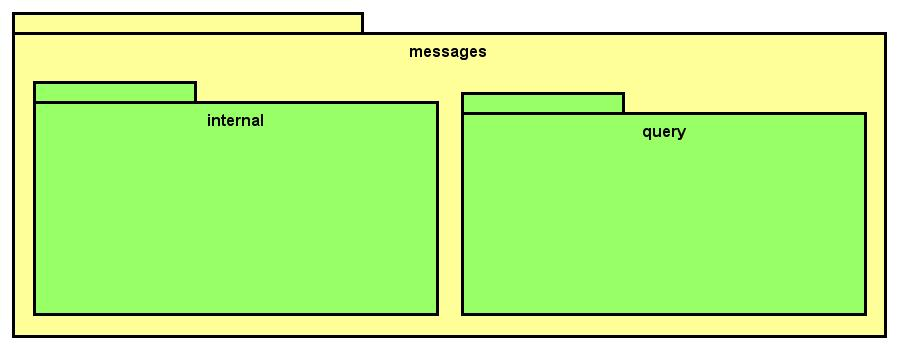
\includegraphics[width=\textwidth]{ST/Server/messagesLevel.jpg}
				\caption{Componente Actorbase.server.messages}
			\end{figure}
			
			\subsubsection{Descrizione}
				Package contenente tutti i messaggi che gli attori si scambiano tra di loro.
				È composto dai package \textbf{internal} e \textbf{query}.
				
			\subsubsection{Package Figli}
				\begin{itemize}
					\item Actorbase.server.messages.internal.
					\item Actorbase.server.messages.query.
				\end{itemize}
				
		\subsection{Actorbase.server.messages.internal}
		
			\begin{figure} [H]
				\centering
				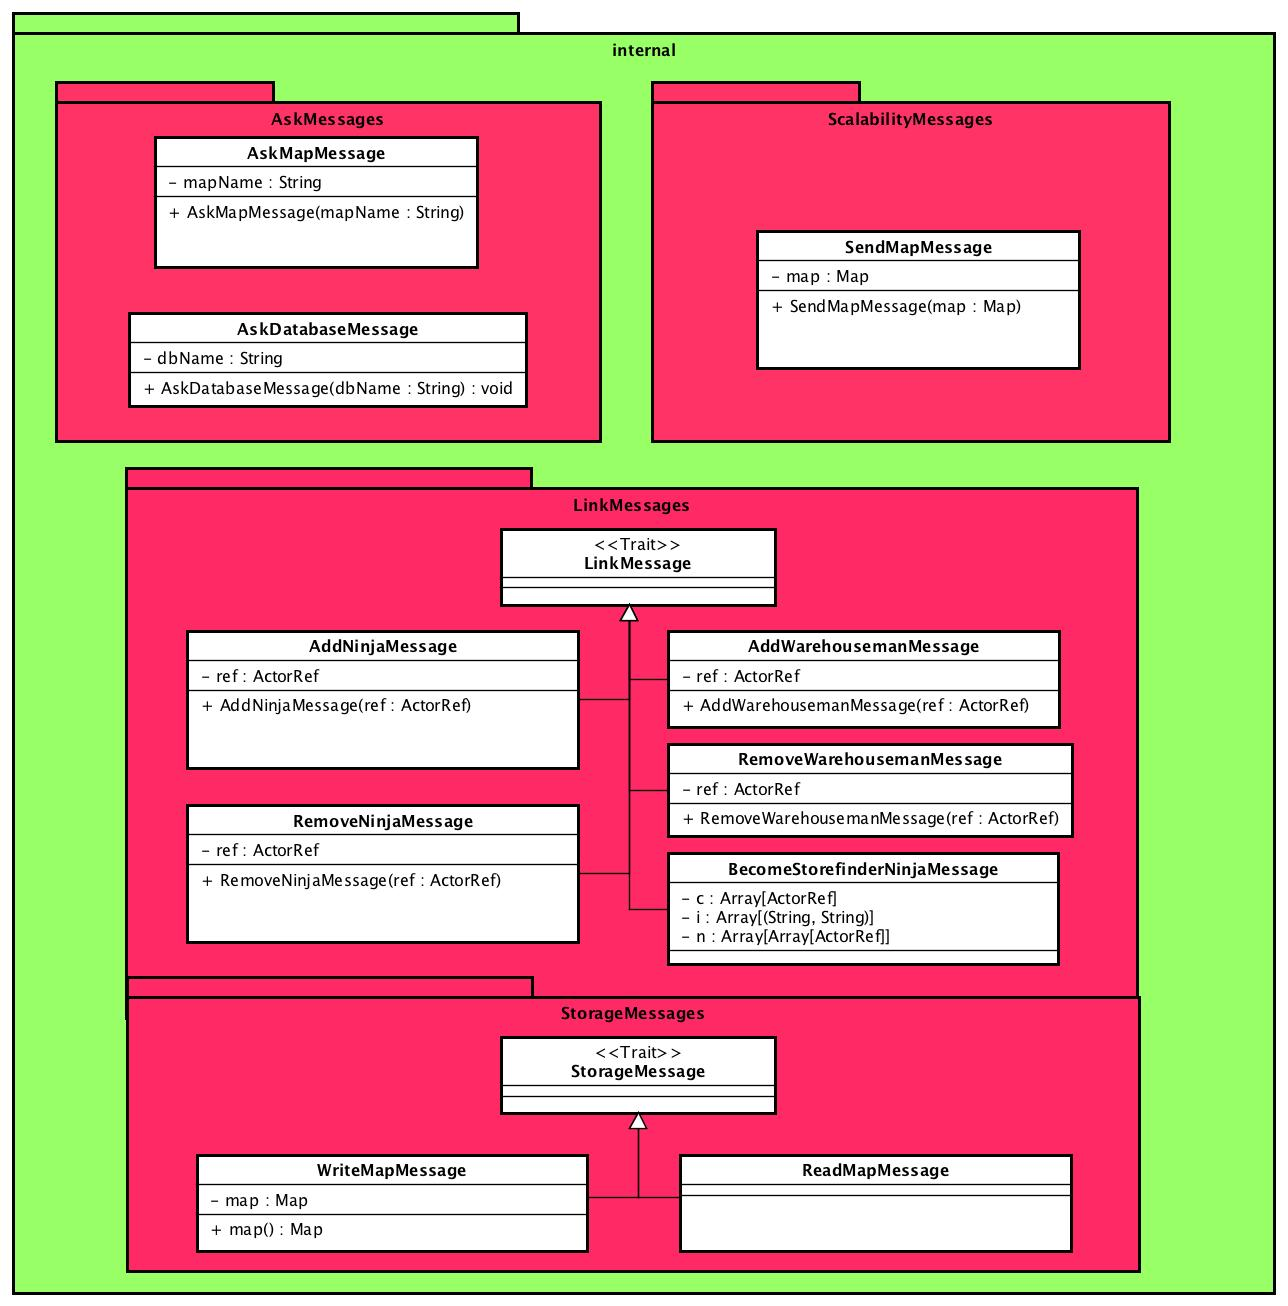
\includegraphics[width=\textwidth]{ST/Server/internalLevel.jpg}
				\caption{Componente Actorbase.server.messages.internal}
			\end{figure}
			
			\subsubsection{Descrizione}
				Package contenente i messaggi che gli attori si scambiano non riguardanti richieste effettuate dagli utenti.
				
			\subsubsection{Package Figli}
				\begin{itemize}
					\item Actorbase.server.messages.internal.LinkMessages
				\end{itemize}
				
			\subsubsection{Classi}
				\begin{itemize}
					\item Actorbase.server.messages.internal.AskMapMessage
					\item Actorbase.server.messages.internal.BecomeStorekeeperMessage
					\item Actorbase.server.messages.internal.SendMapMessage
				\end{itemize}
			
		\subsection{Actorbase.server.messages.internal.AskMapMessage}
			\subsubsection{Descrizione}
				Questa classe rappresenta un messaggio per verificare la presenza di una mappa in un \textbf{Storemanager}.
				
			\subsubsection{Utilizzo}
				Viene inviato da un \textbf{Main} ad uno \textbf{Storemanager}.
				
			\subsubsection{Relazione con altre classi}
				\begin{itemize}
					\item \textbf{Actorbase.server.actors.Main:} relazione entrante, creazione e utilizzo.
					\item \textbf{Actorbase.server.actors.Storemanager:} relazione di utilizzo.
				\end{itemize}
				
		\subsection{Actorbase.server.messages.internal.BecomeAStorekeeperMsg}
			\subsubsection{Descrizione}
				Questa classe rappresenta un messaggio per far cambiare l'implementazione di ricezione di messaggi di uno \textbf{Storekeeper} 
				che precedentemente si comportava come un \textbf{Ninja}.
				
			\subsubsection{Utilizzo}
				Viene inviato da uno \textbf{Storefinder} ad uno \textbf{Storekeeper}.
				
			\subsubsection{Relazione con altre classi}
				\begin{itemize}
					\item \textbf{Actorbase.server.actors.Storefinder:} relazione entrante, creazione e utilizzo.
					\item \textbf{Actorbase.server.actors.Storekeeper:} relazione di utilizzo.
				\end{itemize}
				
		\subsection{Actorbase.server.messages.internal.SendMapMessage}
			\subsubsection{Descrizione}
				Questa classe rappresenta un messaggio contenente una mappa. 
				
			\subsubsection{Utilizzo}
				Viene inviato da un \textbf{Warehouseman} ad uno \textbf{Storekeeper}.
				
			\subsubsection{Relazione con altre classi}
				\begin{itemize}
					\item \textbf{Actorbase.server.actors.Warehouseman:} relazione entrante, creazione e utilizzo.
					\item \textbf{Actorbase.server.actors.Storekeeper:} relazione di utilizzo.
				\end{itemize}
				
		\subsection{Actorbase.server.messages.internal.LinkMessages}
			
			\subsubsection{Descrizione}
				Package contenente i messaggi che gli attori si scambiano non riguardanti richieste effettuate dagli utenti.
				
			\subsubsection{Classi}
				\begin{itemize}
					\item Actorbase.server.messages.internal.LinkMessages.AddNinjaMessage
					\item Actorbase.server.messages.internal.LinkMessages.AddWarehousemanMessage
					\item Actorbase.server.messages.internal.LinkMessages.RemoveNinjaMessage
					\item Actorbase.server.messages.internal.LinkMessages.RemoveWarehousemanMessage
				\end{itemize}
			
			\subsubsection{Trait}
				\begin{itemize}
					\item Actorbase.server.messages.internal.LinkMessages.LinkMessage
				\end{itemize}
				
		\subsection{Actorbase.server.messages.internal.LinkMessages.LinkMessage}
			\subsubsection{Descrizione}
				Trait per la richiesta di aggiunta o rimozione di un attore da parte di un altro attore.
				
			\subsubsection{Utilizzo}
				Viene inviato da uno \textbf{Storefinder} ad uno \textbf{Storekeeper}.
				
			\subsubsection{Relazione con altre classi}
				\begin{itemize}
					\item \textbf{Actorbase.server.actors.Storefinder:} relazione entrante, creazione e utilizzo.
					\item \textbf{Actorbase.server.actors.Storekeeper:} relazione di utilizzo.
				\end{itemize}
				
			\subsubsection{Classi figlie}
				\begin{itemize}
					\item Actorbase.server.messages.internal.LinkMessages.AddNinjaMessage
					\item Actorbase.server.messages.internal.LinkMessages.AddWarehousemanMessage
					\item Actorbase.server.messages.internal.LinkMessages.RemoveNinjaMessage
					\item Actorbase.server.messages.internal.LinkMessages.RemoveWarehousemanMessage
				\end{itemize}
				
		\subsection{Actorbase.server.messages.internal.LinkMessages.AddNinjaMessage}
			\subsubsection{Descrizione}
				Questa classe rappresenta la richiesta di aggiunta di un \textbf{Ninja}, ovvero uno \textbf{Storekeeper} di backup, da 
				parte di uno \textbf{Storefinder} ad uno \textbf{Storekeeper}.
				
			\subsubsection{Utilizzo}
				Viene inviato da uno \textbf{Storefinder} ad uno \textbf{Storekeeper}.
				
			\subsubsection{Relazione con altre classi}
				\begin{itemize}
					\item \textbf{Actorbase.server.actors.Storefinder:} relazione entrante, creazione e utilizzo.
					\item \textbf{Actorbase.server.actors.Storekeeper:} relazione di utilizzo.
				\end{itemize}
				
			\subsubsection{Trait implementati}
				\begin{itemize}
					\item \textbf{Actorbase.server.messages.internal.LinkMessages.LinkMessage} 
				\end{itemize}
				
		\subsection{Actorbase.server.messages.internal.LinkMessages.AddWarehousemanMessage}
			\subsubsection{Descrizione}
				Questa classe rappresenta la richiesta di aggiunta di un \textbf{Warehouseman} da parte di uno \textbf{Storefinder} 
				ad uno \textbf{Storekeeper}.
				
			\subsubsection{Utilizzo}
				Viene inviato da uno \textbf{Storefinder} ad uno \textbf{Storekeeper}.
				
			\subsubsection{Relazione con altre classi}
				\begin{itemize}
					\item \textbf{Actorbase.server.actors.Storefinder:} relazione entrante, creazione e utilizzo.
					\item \textbf{Actorbase.server.actors.Storekeeper:} relazione di utilizzo.
				\end{itemize}
				
			\subsubsection{Trait implementati}
				\begin{itemize}
					\item \textbf{Actorbase.server.messages.internal.LinkMessages.LinkMessage} 
				\end{itemize}
				
		\subsection{Actorbase.server.messages.internal.LinkMessages.RemoveNinjaMessage}
			\subsubsection{Descrizione}
				Questa classe rappresenta la richiesta di rimozione di un \textbf{Ninja}, ovvero uno \textbf{Storekeeper} di backup, da 
				parte di uno \textbf{Storefinder} ad uno \textbf{Storekeeper}.
				
			\subsubsection{Utilizzo}
				Viene inviato da uno \textbf{Storefinder} ad uno \textbf{Storekeeper}.
				
			\subsubsection{Relazione con altre classi}
				\begin{itemize}
					\item \textbf{Actorbase.server.actors.Storefinder:} relazione entrante, creazione e utilizzo.
					\item \textbf{Actorbase.server.actors.Storekeeper:} relazione di utilizzo.
				\end{itemize}
				
			\subsubsection{Trait implementati}
				\begin{itemize}
					\item \textbf{Actorbase.server.messages.internal.LinkMessages.LinkMessage} 
				\end{itemize}
				
		\subsection{Actorbase.server.messages.internal.LinkMessages.RemoveWarehousemanMessage}
			\subsubsection{Descrizione}
				Questa classe rappresenta la richiesta di rimozione di un \textbf{Warehouseman} da parte di uno \textbf{Storefinder} 
				ad uno \textbf{Storekeeper}.
				
			\subsubsection{Utilizzo}
				Viene inviato da uno \textbf{Storefinder} ad uno \textbf{Storekeeper}.
				
			\subsubsection{Relazione con altre classi}
				\begin{itemize}
					\item \textbf{Actorbase.server.actors.Storefinder:} relazione entrante, creazione e utilizzo.
					\item \textbf{Actorbase.server.actors.Storekeeper:} relazione di utilizzo.
				\end{itemize}
				
			\subsubsection{Trait implementati}
				\begin{itemize}
					\item \textbf{Actorbase.server.messages.internal.LinkMessages.LinkMessage} 
				\end{itemize}
				
		\subsection{Actorbase.server.messages.query}
		
			\begin{figure}[H]
				\centering
				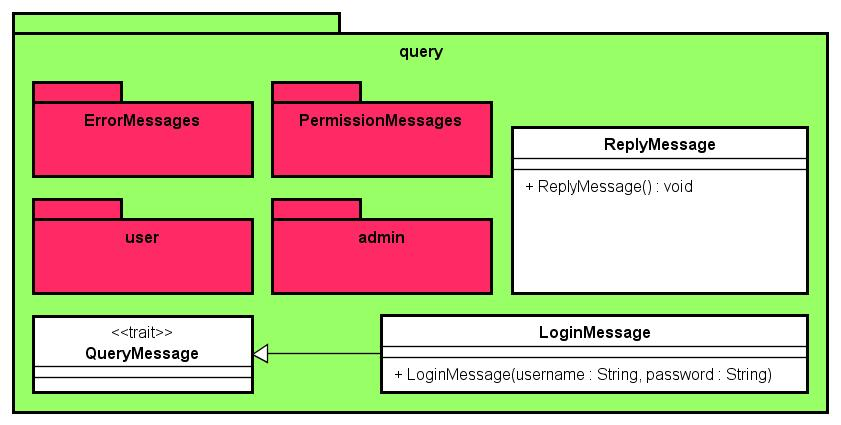
\includegraphics[width=\textwidth]{ST/Server/queryLevel}
				\caption{Componente Actorbase.server.messages.query}
			\end{figure}
			
			\subsubsection{Descrizione}
				Package contenente i messaggi che rappresentano le possibili richieste che gli utenti possono effettuare. Questi messaggi vengono 
				scambiati tra gli attori presenti nel database.
				
			\subsubsection{Package Figli}
				\begin{itemize}
					\item Actorbase.server.messages.query.ErrorMessages
					\item Actorbase.server.messages.query.PermissionMessages
					\item Actorbase.server.messages.query.user
					\item Actorbase.server.messages.query.admin
				\end{itemize}
				
			\subsubsection{Classi}
				\begin{itemize}
					\item Actorbase.server.messages.query.LoginMessage
					\item Actorbase.server.messages.query.ReplyMessage
				\end{itemize}
				
			\subsubsection{Trait}
				\begin{itemize}
					\item Actorbase.server.messages.query.QueryMessage
				\end{itemize}

		\subsection{Actorbase.server.messages.query.QueryMessage}
		\label{QueryMessage}
			\subsubsection{Descrizione}
				Classe che rappresenta un messaggio contenente una richiesta effettuata da un utente.
				
			\subsubsection{Utilizzo}
				Viene utilizzata da tutti gli attori, in particolar modo segue diversi percorsi in base alla sottoclasse concreta a cui appartiene.
				Viene creato da un \textbf{Parser} sotto richiesta di un \textbf{Usermanager} ed inviato ad un \textbf{Main}. Da qui può fermarsi in 
				qualsiasi punto della sequenza: \textbf{Storemanager} \space -> \space \textbf{Storefinder} 
				\space -> \space \textbf{Storekeeper} \space -> \space \textbf{Warehouseman}.
			\subsubsection{Relazioni con altre classi}
				\begin{itemize}
					\item \textbf{Actorbase.server.utils.Parser:} relazione entrante di creazione.
					\item \textbf{Actorbase.server.actors.Usermanager:} relazione di utilizzo.
					\item \textbf{Actorbase.server.actors.Main:} relazione di utilizzo.
					\item \textbf{Actorbase.server.actors.Storemanager:} relazione di utilizzo.
					\item \textbf{Actorbase.server.actors.Storefinder:} relazione di utilizzo.
					\item \textbf{Actorbase.server.actors.Storekeeper:} relazione di utilizzo.
					\item \textbf{Actorbase.server.actors.Warehouseman:} relazione di utilizzo.
					\item \textbf{Actorbase.server.messages.query.ReplyMessage:} relazione entrante, aggregazione.
				\end{itemize}
			\subsubsection{Classi figlie}
				\begin{itemize}
					\item Actorbase.server.messages.query.LoginMessage
					\item Actorbase.server.messages.query.ErrorMessages.InvalidQueryMessage
					\item Actorbase.server.messages.query.admin.AdminMessage
					\item Actorbase.server.messages.query.user.UserMessage
				\end{itemize}
				
		\subsection{Actorbase.server.messages.query.LoginMessage}
			\subsubsection{Descrizione}
				Classe che rappresenta un messaggio contenente la richiesta di login effettuata da parte di un utente.
				
			\subsubsection{Utilizzo}
				Nel percorso esposto in \hyperref[QueryMessage]{Actorbase.server.messages.query.QueryMessage} si ferma all'attore \textbf{Usermanager}.
				
			\subsubsection{Relazioni con altre classi}
				\begin{itemize}
					\item \textbf{Actorbase.server.utils.Parser:} relazione entrante di creazione.
					\item \textbf{Actorbase.server.actors.Usermanager:} relazione di utilizzo.
				\end{itemize}
			\subsubsection{Trait implementati}
				\begin{itemize}
					\item Actorbase.server.messages.query.QueryMessage
				\end{itemize}
		
		\subsection{Actorbase.server.messages.query.ReplyMEssage}
			\subsubsection{Descrizione}
				Classe che rappresenta un messaggio di risposta ad una richiesta effettuata da parte di un utente.
				
			\subsubsection{Utilizzo}
				Effettua il percorso esposto in \hyperref[QueryMessage]{Actorbase.server.messages.query.QueryMessage} in senso opposto.
				
			\subsubsection{Relazioni con altre classi}
				\begin{itemize}
					\item \textbf{Actorbase.server.actors.Usermanager:} relazione entrante, creazione e utilizzo.
					\item \textbf{Actorbase.server.actors.Main:} relazione entrante, creazione e utilizzo.
					\item \textbf{Actorbase.server.actors.Storemanager:} relazione entrante, creazione e utilizzo.
					\item \textbf{Actorbase.server.actors.Storefinder:} relazione entrante, creazione e utilizzo.
					\item \textbf{Actorbase.server.actors.Storekeeper:} relazione entrante, creazione e utilizzo.
					\item \textbf{Actorbase.server.actors.Warehouseman:} relazione entrante, creazione e utilizzo.
				\end{itemize}
				
		\subsection{Actorbase.server.messages.query.ErrorMessages}
		
			\begin{figure}[H]
				\centering
				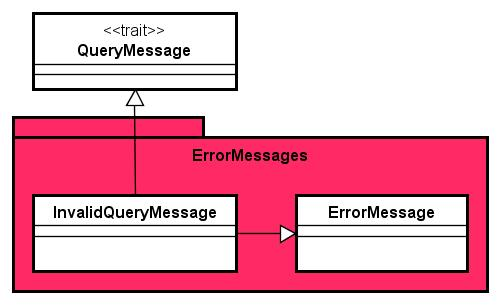
\includegraphics[width=\textwidth]{ST/Server/errorMessagesLevel}
				\caption{Componente Actorbase.server.messages.query.ErrorMessages}
			\end{figure}
			
			\subsubsection{Descrizione}
				Package contenente i messaggi di errore che vengono utilizzati qualora si verifichi un errore durante la 
				realizzazione di una richiesta effettuata da un utente.
				
			\subsubsection{Classi}
				\begin{itemize}
					\item Actorbase.server.messages.query.ErrorMessages.InvalidQueryMessage
				\end{itemize}
				
			\subsubsection{Trait}
				\begin{itemize}
					\item Actorbase.server.messages.query.ErrorMessages.ErrorMessage
				\end{itemize}
				
		\subsection{Actorbase.server.messages.query.ErrorMessages.ErrorMessage}
			\subsubsection{Descrizione}
				Trait per segnalare che la richiesta effettuata non è riconosciuta dal server.
				
			\subsubsection{Utilizzo}
				Viene inviato da uno \textbf{Usermanager}.
				
			\subsubsection{Relazione con altre classi}
				\begin{itemize}
					\item \textbf{Actorbase.server.actors.Usermanager:} relazione entrante, creazione e utilizzo.
					\item \textbf{Actorbase.server.utils.Parser:} relazione entrante, creazione.
				\end{itemize}
				
			\subsubsection{Classi figlie}
				\begin{itemize}
					\item Actorbase.server.messages.query.ErrorMessages.InvalidQueryMessage
				\end{itemize}
				
		\subsection{Actorbase.server.messages.query.ErrorMessages.InvalidQueryMessage}
			\subsubsection{Descrizione}
				Questa classe rappresenta un messaggio per segnalare che la richiesta effettuata non è riconosciuta dal server.
				
			\subsubsection{Utilizzo}
				Viene inviato da uno \textbf{Usermanager}.
				
			\subsubsection{Relazione con altre classi}
				\begin{itemize}
					\item \textbf{Actorbase.server.actors.Usermanager:} relazione entrante, creazione e utilizzo.
					\item \textbf{Actorbase.server.utils.Parser:} relazione entrante, creazione.
				\end{itemize}
			
			\subsubsection{Trait implementati}
				\begin{itemize}
					\item \textbf{Actorbase.server.messages.query.QueryMessage}
					\item \textbf{Actorbase.server.messages.query.ErrorMessages.ErrorMessage} 
				\end{itemize}

		\subsection{Actorbase.server.messages.query.PermissionMessages}
		
			\begin{figure}[H]
				\centering
				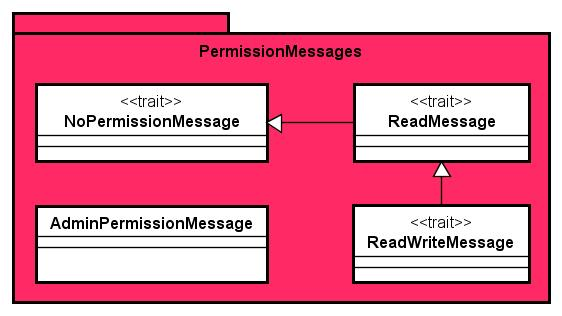
\includegraphics[width=\textwidth]{ST/Server/permissionMessagesLevel}
				\caption{Componente Actorbase.server.messages.query.PermissionMessages}
			\end{figure}
			
			\subsubsection{Descrizione}
				Package contenente i messaggi che rappresentano i vari livelli di permessi necessari agli utenti al fine di poter 
				effettuare una richiesta.
				
			\subsubsection{Trait}
				\begin{itemize}
					\item Actorbase.server.messages.query.PermissionMessages.AdminPermissionMessage
					\item Actorbase.server.messages.query.PermissionMessages.NoPermissionMessage
					\item Actorbase.server.messages.query.PermissionMessages.ReadMessage
					\item Actorbase.server.messages.query.PermissionMessages.ReadWrite
				\end{itemize}
				
		\subsection{Actorbase.server.messages.query.PermissionMessages.AdminPermissionMessage}
			\subsubsection{Descrizione}
				Trait che rappresenta un comando che richiede i permessi di amministrazione per la sua esecuzione.
				
			\subsubsection{Utilizzo}
				Ha lo stesso utilizzo di \hyperref[QueryMessage]{Actorbase.server.messages.query.QueryMessage}.
				
			\subsubsection{Classi figlie}
				\begin{itemize}
					\item Actorbase.server.messages.query.admin.AdminMessage
				\end{itemize}
		
		\subsection{Actorbase.server.messages.query.PermissionMessages.NoPermissionMessage}
			\subsubsection{Descrizione}
				Trait che rappresenta un comando che non richiede alcun permesso per la sua esecuzione.
				
			\subsubsection{Utilizzo}
				Ha lo stesso utilizzo di \hyperref[QueryMessage]{Actorbase.server.messages.query.QueryMessage}.
				
			\subsubsection{Classi figlie}
				\begin{itemize}
					\item Actorbase.server.messages.query.user.DatabaseMessages.CreateDatabaseMessage
					\item Actorbase.server.messages.query.user.HelpMessages.CompleteHelpMessage
					\item Actorbase.server.messages.query.user.HelpMessages.SpecificHelpMessage
				\end{itemize}
				
		\subsection{Actorbase.server.messages.query.PermissionMessages.ReadMessage}
			\subsubsection{Descrizione}
				Trait che rappresenta un comando che richiede almeno i permessi di lettura per la sua esecuzione.
				
			\subsubsection{Utilizzo}
				Ha lo stesso utilizzo di \hyperref[QueryMessage]{Actorbase.server.messages.query.QueryMessage}.
				
			\subsubsection{Classi figlie}
				\begin{itemize}
					\item Actorbase.server.messages.query.user.DatabaseMessages.SelectDatabaseMessage
					\item Actorbase.server.messages.query.user.DatabaseMessages.ListDatabaseMessage
					\item Actorbase.server.messages.query.user.MapMessages.SelectMapMessage
					\item Actorbase.server.messages.query.user.MapMessages.ListMapMessage
					\item Actorbase.server.messages.query.user.RowMessages.FindRowMessage
					\item Actorbase.server.messages.query.user.RowMessages.ListKeysMessage
				\end{itemize}
				
		\subsection{Actorbase.server.messages.query.PermissionMessages.ReadWriteMessage}
			\subsubsection{Descrizione}
				Trait che rappresenta un comando che richiede i permessi di scrittura per la sua esecuzione.
				
			\subsubsection{Utilizzo}
				Ha lo stesso utilizzo di \hyperref[QueryMessage]{Actorbase.server.messages.query.QueryMessage}.
				
			\subsubsection{Classi figlie}
				\begin{itemize}
					\item Actorbase.server.messages.query.user.DatabaseMessages.DeleteDatabaseMessage
					\item Actorbase.server.messages.query.user.MapMessages.DeleteMapMessage
					\item Actorbase.server.messages.query.user.MapMessages.CreateMapMessage
					\item Actorbase.server.messages.query.user.RowMessages.InsertRowMessage
					\item Actorbase.server.messages.query.user.RowMessages.UpdateRowMessage
					\item Actorbase.server.messages.query.user.RowMessages.RemoveRowMessage
				\end{itemize}
				
		\subsection{Actorbase.server.messages.query.admin}
		
			\begin{figure}[H]
				\centering
				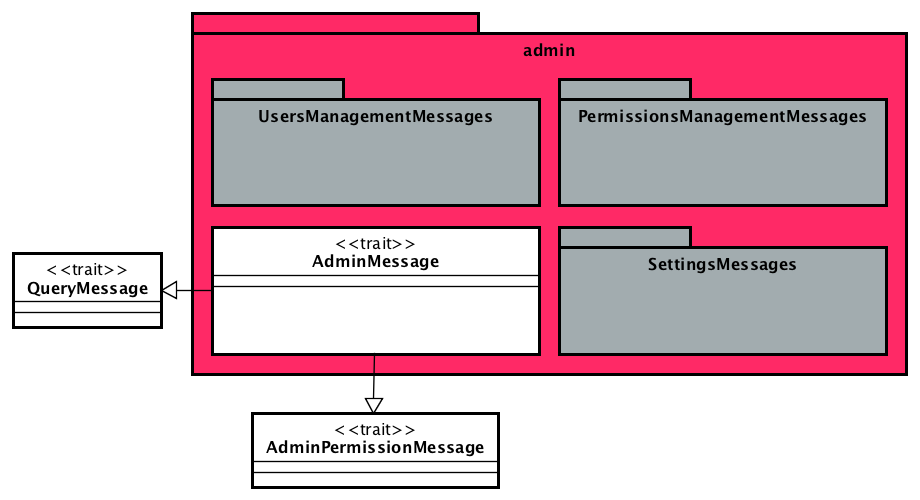
\includegraphics[width=\textwidth]{ST/Server/adminLevel}
				\caption{Componente Actorbase.server.messages.query.admin}
			\end{figure}
			
			\subsubsection{Descrizione}
				Package contenente i messaggi che rappresentano i comandi amministrativi.
				
			\subsubsection{Package Figli}
				\begin{itemize}
					\item Actorbase.server.messages.query.admin.ActorPropertiesMessages
					\item Actorbase.server.messages.query.admin.PermissionsManagementMessages
					\item Actorbase.server.messages.query.admin.UserManagementMessages
				\end{itemize}
				
			\subsubsection{Trait}
				\begin{itemize}
					\item Actorbase.server.messages.query.admin.AdminMessage
				\end{itemize}
				
		\subsection{Actorbase.server.messages.query.admin.AdminMessage}
			\subsubsection{Descrizione}
				Trait che rappresenta tutti i comandi per effettuare operazioni di tipo amministrativo.
				
			\subsubsection{Utilizzo}
				Viene utilizzato per poter distinguere i comandi di tipo amministrativo da altri comandi.
				
			\subsubsection{Relazioni con altre classi}
				\begin{itemize}
					\item \textbf{Actorbase.server.utils.Parser:} relazione entrante di creazione.
					\item \textbf{Actorbase.server.actors.Usermanager:} relazione di utilizzo.
					\item \textbf{Actorbase.server.actors.Main:} relazione di utilizzo.
				\end{itemize}
			\subsubsection{Classi figlie}
				\begin{itemize}
					\item Actorbase.server.messages.query.admin.ActorPropertiesMessage
					\item Actorbase.server.messages.query.admin.PermissionsManagementMessage
					\item Actorbase.server.messages.query.admin.UsersManagementMessage
				\end{itemize}
		
		\subsection{Actorbase.server.messages.query.admin.ActorPropertiesMessages}
		
			\begin{figure}[H]
				\centering
				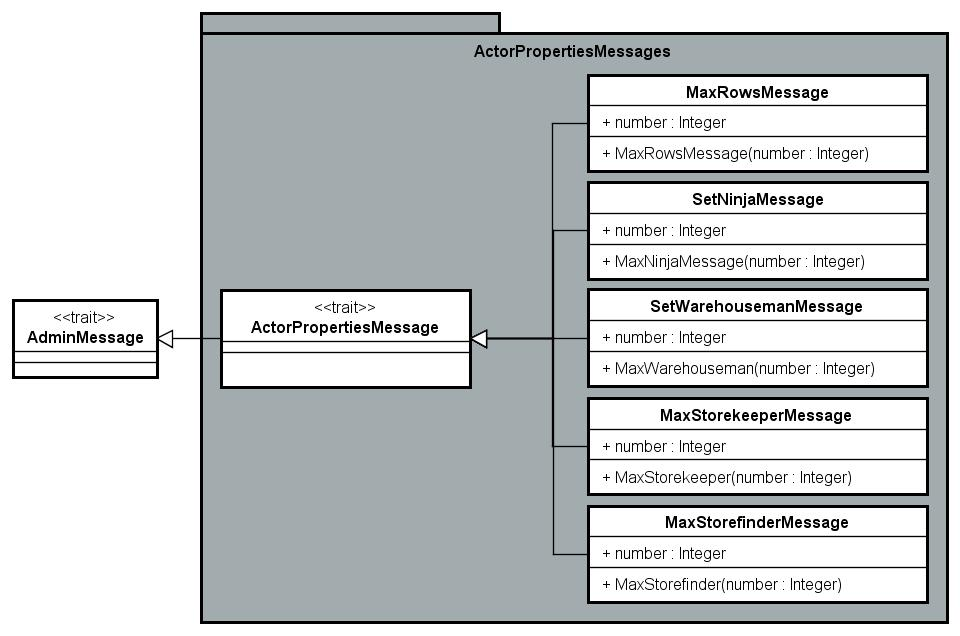
\includegraphics[width=\textwidth]{ST/Server/actorPropertiesLevel.jpg}
				\caption{Componente Actorbase.server.messages.query.admin.ActorPropertiesMessages}
			\end{figure}
			
			\subsubsection{Descrizione}
				Package contenente i messaggi per modificare le proprietà degli attori che compongono il sistema.
				
			\subsubsection{Classi}
				\begin{itemize}
					\item Actorbase.server.messages.query.admin.ActorPropertiesMessages.MaxRowMessage
					\item Actorbase.server.messages.query.admin.ActorPropertiesMessages.MaxNinjaMessage
					\item Actorbase.server.messages.query.admin.ActorPropertiesMessages.SetWarehousemanMessage
					\item Actorbase.server.messages.query.admin.ActorPropertiesMessages.MaxStorekeeperMessage
					\item Actorbase.server.messages.query.admin.ActorPropertiesMessages.MaxStorefinderMessage
				\end{itemize}
				
			\subsubsection{Trait}
				\begin{itemize}
					\item Actorbase.server.messages.query.admin.ActorPropertiesMessages.ActorPropertiesMessage
				\end{itemize}
		
		\subsection{Actorbase.server.messages.query.admin \newline .ActorPropertiesMessages.ActorPropertiesMessage}
			\subsubsection{Descrizione}
				Trait per identificare i messaggi per modificare le proprietà degli attori che compongono il sistema.
				
			\subsubsection{Utilizzo}
				Viene utilizzato per poter distinguere i comandi per modificare le proprietà degli attori che compongono il sistema.
				
			\subsubsection{Relazioni con altre classi}
				\begin{itemize}
					\item \textbf{Actorbase.server.utils.Parser:} relazione entrante di creazione.
					\item \textbf{Actorbase.server.actors.Usermanager:} relazione di utilizzo.
					\item \textbf{Actorbase.server.actors.Main:} relazione di utilizzo.
					\item \textbf{Actorbase.server.actors.Storemanager:} relazione entrante, creazione e utilizzo.
					\item \textbf{Actorbase.server.actors.Storefinder:} relazione entrante, creazione e utilizzo.
					\item \textbf{Actorbase.server.actors.Storekeeper:} relazione entrante, creazione e utilizzo.
					\item \textbf{Actorbase.server.actors.Warehouseman:} relazione entrante, creazione e utilizzo.
				\end{itemize}
			\subsubsection{Classi figlie}
				\begin{itemize}
					\item Actorbase.server.messages.query.admin.ActorPropertiesMessages.MaxRowMessage
					\item Actorbase.server.messages.query.admin.ActorPropertiesMessages.SetNinjaMessage
					\item Actorbase.server.messages.query.admin.ActorPropertiesMessages.SetWarehousemanMessage
					\item Actorbase.server.messages.query.admin.ActorPropertiesMessages.MaxStorekeeperMessage
					\item Actorbase.server.messages.query.admin.ActorPropertiesMessages.MaxStorefinderMessage
				\end{itemize}

		\subsection{Actorbase.server.messages.query.admin \newline
		.ActorPropertiesMessages.MaxRowMessage}
		
			\subsubsection{Descrizione}
				Questa classe rappresenta un messaggio per modificare il numero di righe massimo di una mappa che uno \textbf{Storekeeper} può gestire.
				
			\subsubsection{Utilizzo}
				Effettua il percorso descritto in \hyperref[QueryMessage]{Actorbase.server.messages.query.QueryMessage} fermandosi all'attore 
				\textbf{Storekeeper}.
				
			\subsubsection{Trait implementati}
				\begin{itemize}
					\item Actorbase.server.messages.query.admin.ActorPropertiesMessages.ActorPropertiesMessage
				\end{itemize}
		
<<<<<<< Updated upstream
		\subsection{Actorbase.server.messages.query.admin.ActorPropertiesMessages.SetNinjaMessage}
=======
		\subsection{Actorbase.server.messages.query.admin \newline
		.ActorPropertiesMessages.MaxNinjaMessage}
>>>>>>> Stashed changes
			\subsubsection{Descrizione}
				Questa classe rappresenta un messaggio per modificare il numero di attori \textbf{Ninja} assegnati ad ogni \textbf{Storekeeper}.
				
			\subsubsection{Utilizzo}
				Effettua il percorso descritto in \hyperref[QueryMessage]{Actorbase.server.messages.query.QueryMessage} fermandosi all'attore 
				\textbf{Storefinder}.
				
			\subsubsection{Relazioni con altre classi}
				\begin{itemize}
					\item \textbf{Actorbase.server.utils.Parser:} relazione entrante di creazione.
					\item \textbf{Actorbase.server.actors.Usermanager:} relazione di utilizzo.
					\item \textbf{Actorbase.server.actors.Main:} relazione di utilizzo.
					\item \textbf{Actorbase.server.actors.Storemanager:} relazione entrante, creazione e utilizzo.
					\item \textbf{Actorbase.server.actors.Storefinder:} relazione entrante, creazione e utilizzo.
				\end{itemize}
			\subsubsection{Trait implementati}
				\begin{itemize}
					\item Actorbase.server.messages.query.admin.ActorPropertiesMessage
				\end{itemize}

<<<<<<< Updated upstream
		\subsection{Actorbase.server.messages.query.admin.ActorPropertiesMessages.SetWarehousemanMessage}
=======
		\subsection{Actorbase.server.messages.query.admin \newline
		.ActorPropertiesMessages.MaxWarehousemanMessage}
>>>>>>> Stashed changes
			\subsubsection{Descrizione}
				Questa classe rappresenta un messaggio per modificare il numero di attori \textbf{Warehouseman} assegnati ad ogni \textbf{Storekeeper}.
				
			\subsubsection{Utilizzo}
				Effettua il percorso descritto in \hyperref[QueryMessage]{Actorbase.server.messages.query.QueryMessage} fermandosi all'attore 
				\textbf{Storefinder}.
				
			\subsubsection{Relazioni con altre classi}
				\begin{itemize}
					\item \textbf{Actorbase.server.utils.Parser:} relazione entrante di creazione.
					\item \textbf{Actorbase.server.actors.Usermanager:} relazione di utilizzo.
					\item \textbf{Actorbase.server.actors.Main:} relazione di utilizzo.
					\item \textbf{Actorbase.server.actors.Storemanager:} relazione entrante, creazione e utilizzo.
					\item \textbf{Actorbase.server.actors.Storefinder:} relazione entrante, creazione e utilizzo.
				\end{itemize}
			\subsubsection{Trait implementati}
				\begin{itemize}
					\item Actorbase.server.messages.query.admin.ActorPropertiesMessage
				\end{itemize}
		
		\subsection{Actorbase.server.messages.query.admin \newline
		.ActorPropertiesMessages.MaxStorekeeperMessage}
			\subsubsection{Descrizione}
				Questa classe rappresenta un messaggio per modificare il numero massimo di attori \textbf{Storekeeper} gestiti da ogni \textbf{Storefinder}.
				
			\subsubsection{Utilizzo}
				Effettua il percorso descritto in \hyperref[QueryMessage]{Actorbase.server.messages.query.QueryMessage} fermandosi all'attore 
				\textbf{Storemanager}.
				
			\subsubsection{Relazioni con altre classi}
				\begin{itemize}
					\item \textbf{Actorbase.server.utils.Parser:} relazione entrante di creazione.
					\item \textbf{Actorbase.server.actors.Usermanager:} relazione di utilizzo.
					\item \textbf{Actorbase.server.actors.Main:} relazione di utilizzo.
					\item \textbf{Actorbase.server.actors.Storemanager:} relazione entrante, creazione e utilizzo.
				\end{itemize}
			\subsubsection{Trait implementati}
				\begin{itemize}
					\item Actorbase.server.messages.query.admin.ActorPropertiesMessage
				\end{itemize}
				
		\subsection{Actorbase.server.messages.query.admin \newline
		.ActorPropertiesMessages.MaxStorefinderMessage}
			\subsubsection{Descrizione}
				Questa classe rappresenta un messaggio per modificare il numero massimo di attori \textbf{Storefinder} gestiti da ogni \textbf{Usermanager}.
				
			\subsubsection{Utilizzo}
				Effettua il percorso descritto in \hyperref[QueryMessage]{Actorbase.server.messages.query.QueryMessage} fermandosi all'attore 
				\textbf{Main}.
				
			\subsubsection{Relazioni con altre classi}
				\begin{itemize}
					\item \textbf{Actorbase.server.utils.Parser:} relazione entrante di creazione.
					\item \textbf{Actorbase.server.actors.Usermanager:} relazione di utilizzo.
					\item \textbf{Actorbase.server.actors.Main:} relazione di utilizzo.
				\end{itemize}
			\subsubsection{Trait implementati}
				\begin{itemize}
					\item Actorbase.server.messages.query.admin.ActorPropertiesMessage
				\end{itemize}
				
		\subsection{Actorbase.server.messages.query.admin.PermissionsManagementMessages}
		
			\begin{figure}[H]
				\centering
				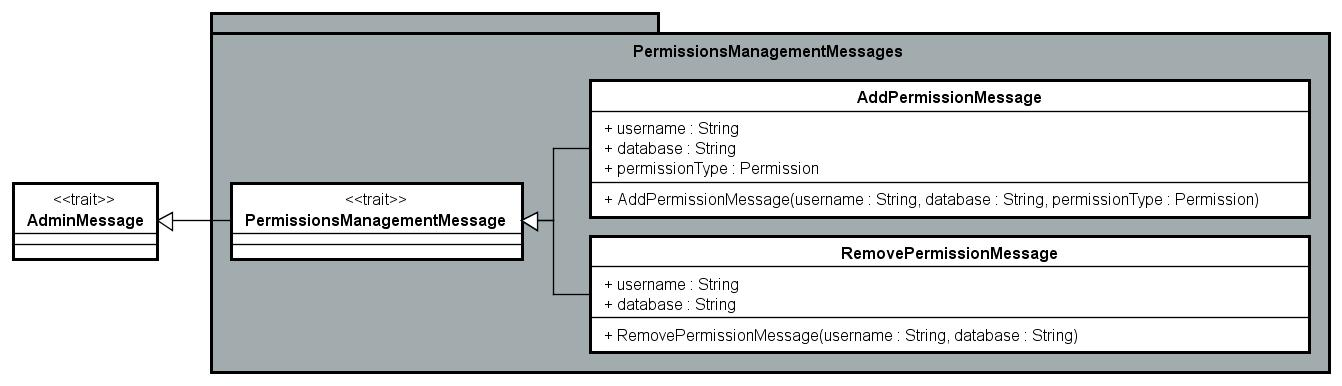
\includegraphics[width=\textwidth]{ST/Server/userPermissionsManagementLevel.jpg}
				\caption{Componente Actorbase.server.messages.query.admin.PermissionsManagementMessages}
			\end{figure}
			
			\subsubsection{Descrizione}
				Pacchetto contenente i messaggi che permettono di gestire i permessi assegnati agli utenti.
			\subsubsection{Classi}
				\begin{itemize}
					\item Actorbase.server.messages.query.admin.PermissionsManagementMessages.AddPermissionMessage
					\item Actorbase.server.messages.query.admin.PermissionsManagementMessages.RemovePermissionMessage
					\item Actorbase.server.messages.query.admin.PermissionsManagementMessages.ListPermissionMessage
				\end{itemize}
				
			\subsubsection{Trait}
				\begin{itemize}
					\item Actorbase.server.messages.query.admin.PermissionsManagementMessages.PermissionsManagementMessage
				\end{itemize}
		
		\subsection{Actorbase.server.messages.query.admin \newline
		.PermissionsManagementMessages.PermissionsManagementMessage}
			\subsubsection{Descrizione}
				Trait che rappresenta i messaggi per gestire i permessi assegnati agli utenti.
				
			\subsubsection{Utilizzo}
				Viene utilizzato per distinguere i messaggi per gestire i permessi assegnati agli utenti.
			\subsubsection{Relazioni con altre classi}
				\begin{itemize}
					\item \textbf{Actorbase.server.utils.Parser:} relazione entrante di creazione.
					\item \textbf{Actorbase.server.actors.Usermanager:} relazione di utilizzo.
					\item \textbf{Actorbase.server.actors.Main:} relazione di utilizzo.
				\end{itemize}
			\subsubsection{Classi figlie}
				\begin{itemize}
					\item Actorbase.server.messages.query.admin.PermissionsManagementMessages.AddPermissionMessage
					\item Actorbase.server.messages.query.admin.PermissionsManagementMessages.RemovePermissionMessage
					\item Actorbase.server.messages.query.admin.PermissionsManagementMessages.ListPermissionMessage
				\end{itemize}
			
		\subsection{Actorbase.server.messages.query.admin \newline
		.PermissionsManagementMessages.AddPermissionMessage}
			\subsubsection{Descrizione}
				Classe che rappresenta un messaggio contenente la richiesta di aggiunta di permessi ad uno specifico utente.
				
			\subsubsection{Utilizzo}
				Viene utilizzata per aggiungere permessi ad uno specifico utente.
				
			\subsubsection{Relazioni con altre classi}
				\begin{itemize}
					\item \textbf{Actorbase.server.utils.Parser:} relazione entrante di creazione.
					\item \textbf{Actorbase.server.actors.Usermanager:} relazione di utilizzo.
					\item \textbf{Actorbase.server.actors.Main:} relazione di utilizzo.
				\end{itemize}
			\subsubsection{Trait implementati}
				\begin{itemize}
					\item Actorbase.server.messages.query.admin.PermissionsManagementMessages.PermissionsManagementMessage
				\end{itemize}
		
		\subsection{Actorbase.server.messages.query.admin \newline
		.PermissionsManagementMessages.RemovePermissionMessage}
			\subsubsection{Descrizione}
				Classe che rappresenta un messaggio contenente la richiesta di rimozione di permessi ad uno specifico utente.
				
			\subsubsection{Utilizzo}
				Viene utilizzata per rimuovere permessi ad uno specifico utente.
				
			\subsubsection{Relazioni con altre classi}
				\begin{itemize}
					\item \textbf{Actorbase.server.utils.Parser:} relazione entrante di creazione.
					\item \textbf{Actorbase.server.actors.Usermanager:} relazione di utilizzo.
					\item \textbf{Actorbase.server.actors.Main:} relazione di utilizzo.
				\end{itemize}
			\subsubsection{Trait implementati}
				\begin{itemize}
					\item Actorbase.server.messages.query.admin.PermissionsManagementMessages.PermissionsManagementMessage
				\end{itemize}
				
		\subsection{Actorbase.server.messages.query.admin \newline
		.PermissionsManagementMessages.ListPermissionMessage}
			\subsubsection{Descrizione}
				Classe che rappresenta un messaggio contenente la richiesta di visualizzazione di permessi di uno specifico utente.
				
			\subsubsection{Utilizzo}
				Viene utilizzata per mostrare i  permessi per ogni database di uno specifico utente.
				
			\subsubsection{Relazioni con altre classi}
				\begin{itemize}
					\item \textbf{Actorbase.server.utils.Parser:} relazione entrante di creazione.
					\item \textbf{Actorbase.server.actors.Usermanager:} relazione di utilizzo.
					\item \textbf{Actorbase.server.actors.Main:} relazione di utilizzo.
				\end{itemize}
			\subsubsection{Trait implementati}
				\begin{itemize}
					\item Actorbase.server.messages.query.admin.PermissionsManagementMessages.PermissionsManagementMessage
				\end{itemize}
				
		\subsection{Actorbase.server.messages.query.admin.UserManagementMessages}
		
			\begin{figure}[H]
				\centering
				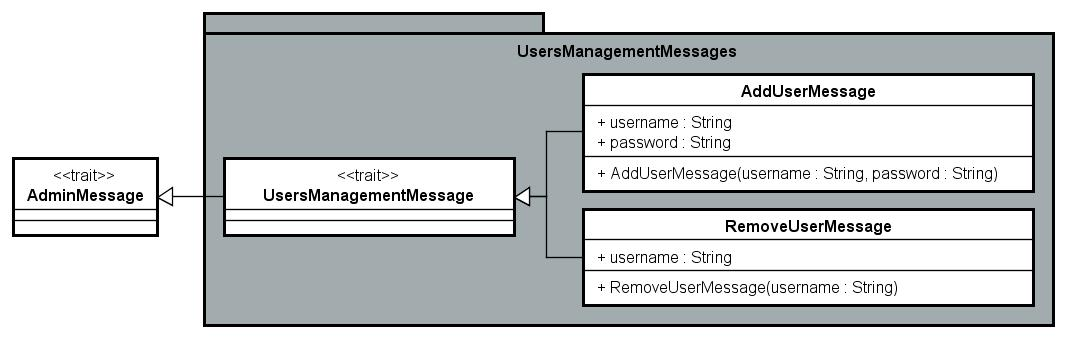
\includegraphics[width=\textwidth]{ST/Server/userManagementLevel.jpg}
				\caption{Componente Actorbase.server.messages.query.admin.UserManagementMessages}
			\end{figure}
			
			\subsubsection{Descrizione}
				Pacchetto contenente i messaggi per gestire gli utenti nel database.
				
			\subsubsection{Classi}
				\begin{itemize}
					\item Actorbase.server.messages.query.admin.UserManagementMessages.AddUserMessage
					\item Actorbase.server.messages.query.admin.UserManagementMessages.RemoveUserMessage
					\item Actorbase.server.messages.query.admin.UserManagementMessages.ListUserMessage
				\end{itemize}
				
			\subsubsection{Trait}
				\begin{itemize}
					\item Actorbase.server.messages.query.admin.UserManagementMessages.UserManagementMessage
				\end{itemize}
				
		\subsection{Actorbase.server.messages.query.admin \newline
		.UserManagementMessages.UserManagementMessage}
			\subsubsection{Descrizione}
				Trait che rappresenta i messaggi per gestire gli utenti nel database.
				
			\subsubsection{Utilizzo}
				Viene utilizzato per distinguere i messaggi per gestire gli utenti nel database.
				
			\subsubsection{Relazioni con altre classi}
				\begin{itemize}
					\item \textbf{Actorbase.server.utils.Parser:} relazione entrante di creazione.
					\item \textbf{Actorbase.server.actors.Usermanager:} relazione di utilizzo.
					\item \textbf{Actorbase.server.actors.Main:} relazione di utilizzo.
				\end{itemize}
			\subsubsection{Classi figlie}
				\begin{itemize}
					\item Actorbase.server.messages.query.admin.UserManagementMessages.AddUserMessage
					\item Actorbase.server.messages.query.admin.UserManagementMessages.RemoveUserMessage
					\item Actorbase.server.messages.query.admin.UserManagementMessages.ListUserMessage
				\end{itemize}
			
		\subsection{Actorbase.server.messages.query.admin \newline
		.UserManagementMessages.AddUserMessage}
			\subsubsection{Descrizione}
				Classe che rappresenta un messaggio contenente la richiesta di aggiunta di un utente.
				
			\subsubsection{Utilizzo}
				Viene utilizzata per aggiungere un utente al sistema.
				
			\subsubsection{Relazioni con altre classi}
				\begin{itemize}
					\item \textbf{Actorbase.server.utils.Parser:} relazione entrante di creazione.
					\item \textbf{Actorbase.server.actors.Usermanager:} relazione di utilizzo.
					\item \textbf{Actorbase.server.actors.Main:} relazione di utilizzo.
				\end{itemize}
			\subsubsection{Trait implementati}
				\begin{itemize}
					\item Actorbase.server.messages.query.admin.UserManagementMessages.UserManagementMessage
				\end{itemize}
		
		\subsection{Actorbase.server.messages.query.admin \newline
		.UserManagementMessages.RemoveUserMessage}
			\subsubsection{Descrizione}
				Classe che rappresenta un messaggio contenente la richiesta di rimozione di un utente.
				
			\subsubsection{Utilizzo}
				Viene utilizzata per rimuovere un utente dal sistema.
				
			\subsubsection{Relazioni con altre classi}
				\begin{itemize}
					\item \textbf{Actorbase.server.utils.Parser:} relazione entrante di creazione.
					\item \textbf{Actorbase.server.actors.Usermanager:} relazione di utilizzo.
					\item \textbf{Actorbase.server.actors.Main:} relazione di utilizzo.
				\end{itemize}
			\subsubsection{Trait implementati}
				\begin{itemize}
					\item Actorbase.server.messages.query.admin.UserManagementMessages.UserManagementMessage
				\end{itemize}
				
		\subsection{Actorbase.server.messages.query.admin \newline 
		.UserManagementMessages.ListUserMessage}
			\subsubsection{Descrizione}
				Classe che rappresenta un messaggio contenente la richiesta di visualizzazione di tutti gli utenti presenti.
				
			\subsubsection{Utilizzo}
				Viene utilizzata per visualizzare tutti gli utenti presenti nel sistema.
				
			\subsubsection{Relazioni con altre classi}
				\begin{itemize}
					\item \textbf{Actorbase.server.utils.Parser:} relazione entrante di creazione.
					\item \textbf{Actorbase.server.actors.Usermanager:} relazione di utilizzo.
					\item \textbf{Actorbase.server.actors.Main:} relazione di utilizzo.
				\end{itemize}
			\subsubsection{Trait implementati}
				\begin{itemize}
					\item Actorbase.server.messages.query.admin.UserManagementMessages.UserManagementMessage
				\end{itemize}
			
		\subsection{Actorbase.server.messages.query.user}
		
			\begin{figure}[H]
				\centering
				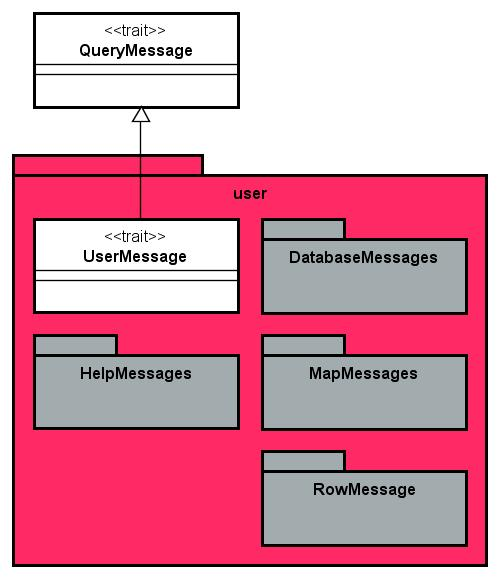
\includegraphics[width=\textwidth]{ST/Server/userLevel.jpg}
				\caption{Componente Actorbase.server.messages.query.user}
			\end{figure}
			
			\subsubsection{Descrizione}
				Pacchetto contenente tutti i messaggi che rappresentano richieste non amministrative.
				
			\subsubsection{Package Figli}
				\begin{itemize}
					\item Actorbase.server.messages.query.user.RowMessages
					\item Actorbase.server.messages.query.user.MapMessages
					\item Actorbase.server.messages.query.user.DatabaseMessages
					\item Actorbase.server.messages.query.user.HelpMessages
				\end{itemize}
				
			\subsubsection{Trait}
				\begin{itemize}
					\item Actorbase.server.messages.query.user.UserMessage
				\end{itemize}
				
		\subsection{Actorbase.server.messages.query.user.UserMessage}
			\subsubsection{Descrizione}
				Trait che rappresenta richieste non amministrative.
				
			\subsubsection{Utilizzo}
				Viene utilizzato per distinguere i messaggi non amministrativi. 
				
			\subsubsection{Relazioni con altre classi}
				\begin{itemize}
					\item \textbf{Actorbase.server.utils.Parser:} relazione entrante di creazione.
					\item \textbf{Actorbase.server.actors.Usermanager:} relazione di utilizzo.
					\item \textbf{Actorbase.server.actors.Main:} relazione di utilizzo.
					\item \textbf{Actorbase.server.actors.Storemanager:} relazione di utilizzo.
					\item \textbf{Actorbase.server.actors.Storefinder:} relazione di utilizzo.
					\item \textbf{Actorbase.server.actors.Storekeeper:} relazione di utilizzo.
					\item \textbf{Actorbase.server.actors.Warehouseman:} relazione di utilizzo.
				\end{itemize}
			\subsubsection{Classi figlie}
				\begin{itemize}
					\item Actorbase.server.messages.query.user.DatabaseMessages.DatabaseMessage
					\item Actorbase.server.messages.query.user.MapMessages.MapMessage
					\item Actorbase.server.messages.query.user.RowMessages.RowMessage
					\item Actorbase.server.messages.query.user.HelpMessages.HelpMessage
				\end{itemize}
		
		\subsection{Actorbase.server.messages.query.user.RowMessages}
		
			\begin{figure}[H]
				\centering
				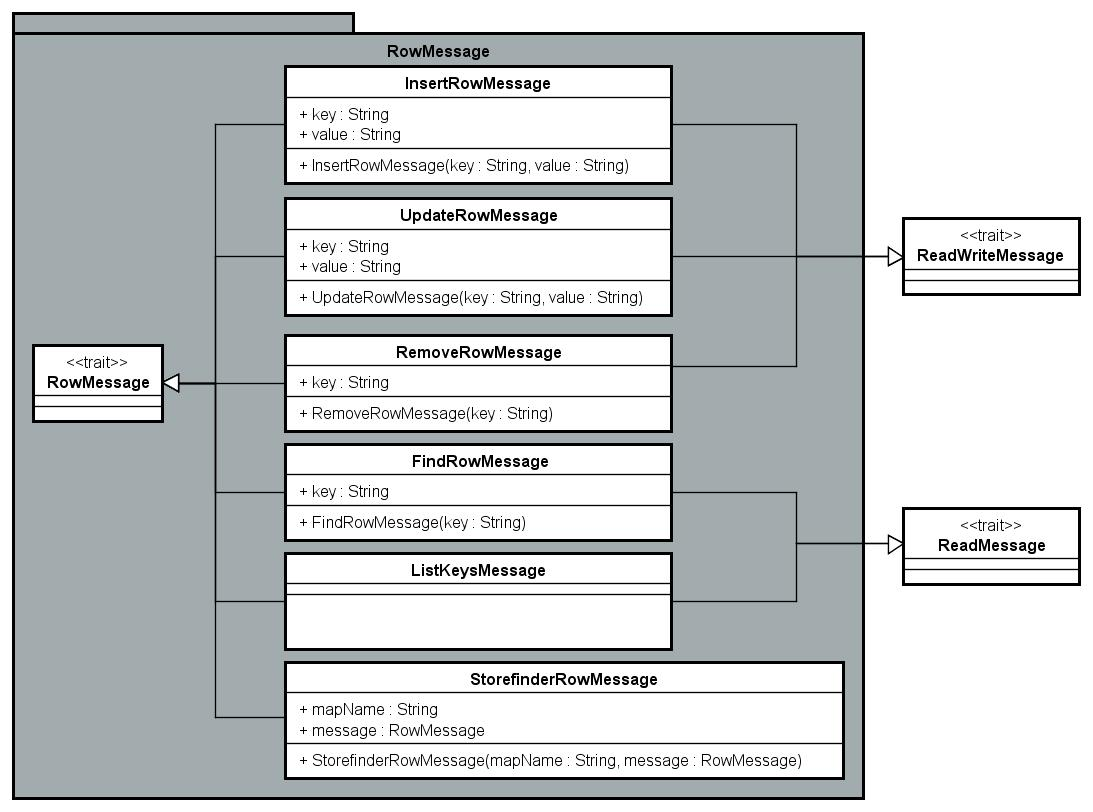
\includegraphics[width=\textwidth]{ST/Server/rowMessagesLevel.jpg}
				\caption{Componente Actorbase.server.messages.query.user.RowMessages}
			\end{figure}
			
			\subsubsection{Descrizione}
				Pacchetto contenente i messaggi che rappresentano le query a livello di riga.
				
			\subsubsection{Classi}
				\begin{itemize}
					\item Actorbase.server.messages.query.user.RowMessages.InsertRowMessage
					\item Actorbase.server.messages.query.user.RowMessages.UpdateRowMessage
					\item Actorbase.server.messages.query.user.RowMessages.RemoveRowMessage
					\item Actorbase.server.messages.query.user.RowMessages.FindRowMessage
					\item Actorbase.server.messages.query.user.RowMessages.ListKeysMessage
				\end{itemize}
				
			\subsubsection{Trait}
				\begin{itemize}
					\item Actorbase.server.messages.query.user.RowMessages.RowMessage
				\end{itemize}
		
		\subsection{Actorbase.server.messages.query.user.RowMessages.RowMessage}
			\subsubsection{Descrizione}
				Trait che rappresenta i messaggi contenenti richieste a livello di riga.
				
			\subsubsection{Utilizzo}
				Viene utilizzato per poter riconoscere i messaggi contenenti richieste a livello di riga.
			\subsubsection{Relazioni con altre classi}
				\begin{itemize}
					\item \textbf{Actorbase.server.utils.Parser:} relazione entrante di creazione.
					\item \textbf{Actorbase.server.actors.Usermanager:} relazione di utilizzo.
					\item \textbf{Actorbase.server.actors.Main:} relazione di utilizzo.
					\item \textbf{Actorbase.server.actors.Storemanager:} relazione di utilizzo.
					\item \textbf{Actorbase.server.actors.Storefinder:} relazione di utilizzo.
					\item \textbf{Actorbase.server.actors.Storekeeper:} relazione di utilizzo.
					\item \textbf{Actorbase.server.actors.Warehouseman:} relazione di utilizzo.
				\end{itemize}
			\subsubsection{Classi figlie}
				\begin{itemize}
					\item Actorbase.server.messages.query.user.RowMessages.InsertRowMessage
					\item Actorbase.server.messages.query.user.RowMessages.UpdateRowMessage
					\item Actorbase.server.messages.query.user.RowMessages.RemoveRowMessage
					\item Actorbase.server.messages.query.user.RowMessages.FindRowMessage
					\item Actorbase.server.messages.query.user.RowMessages.ListKeysMessage
				\end{itemize}
		
		\subsection{Actorbase.server.messages.query.user.RowMessages.InsertRowMessage}
			\subsubsection{Descrizione}
				Classe che rappresenta un messaggio contente la richiesta di inserimento di una riga in una mappa.
				
			\subsubsection{Utilizzo}
				Effettua l'intero percorso descritto in \hyperref[QueryMessage]{Actorbase.server.messages.query.QueryMessage}.
				
			\subsubsection{Relazioni con altre classi}
				\begin{itemize}
					\item \textbf{Actorbase.server.utils.Parser:} relazione entrante di creazione.
					\item \textbf{Actorbase.server.actors.Usermanager:} relazione di utilizzo.
					\item \textbf{Actorbase.server.actors.Main:} relazione di utilizzo.
					\item \textbf{Actorbase.server.actors.Storemanager:} relazione di utilizzo.
					\item \textbf{Actorbase.server.actors.Storefinder:} relazione di utilizzo.
					\item \textbf{Actorbase.server.actors.Storekeeper:} relazione di utilizzo.
					\item \textbf{Actorbase.server.actors.Warehouseman:} relazione di utilizzo.
				\end{itemize}
			\subsubsection{Trait implementati}
				\begin{itemize}
					\item Actorbase.server.messages.query.user.RowMessages.RowMessage
				\end{itemize}
		
		\subsection{Actorbase.server.messages.query.user.RowMessages.UpdateRowMessage}
			\subsubsection{Descrizione}
				Classe che rappresenta un messaggio contente la richiesta di modifica di una riga in una mappa.
				
			\subsubsection{Utilizzo}
				Effettua l'intero percorso descritto in \hyperref[QueryMessage]{Actorbase.server.messages.query.QueryMessage}.
				
			\subsubsection{Relazioni con altre classi}
				\begin{itemize}
					\item \textbf{Actorbase.server.utils.Parser:} relazione entrante di creazione.
					\item \textbf{Actorbase.server.actors.Usermanager:} relazione di utilizzo.
					\item \textbf{Actorbase.server.actors.Main:} relazione di utilizzo.
					\item \textbf{Actorbase.server.actors.Storemanager:} relazione di utilizzo.
					\item \textbf{Actorbase.server.actors.Storefinder:} relazione di utilizzo.
					\item \textbf{Actorbase.server.actors.Storekeeper:} relazione di utilizzo.
					\item \textbf{Actorbase.server.actors.Warehouseman:} relazione di utilizzo.
				\end{itemize}
			\subsubsection{Trait implementati}
				\begin{itemize}
					\item Actorbase.server.messages.query.user.RowMessages.RowMessage
				\end{itemize}
				
		\subsection{Actorbase.server.messages.query.user.RowMessages.RemoveRowMessage}
			\subsubsection{Descrizione}
				Classe che rappresenta un messaggio contente la richiesta di rimozione di una riga in una mappa.
				
			\subsubsection{Utilizzo}
				Effettua l'intero percorso descritto in \hyperref[QueryMessage]{Actorbase.server.messages.query.QueryMessage}.
				
			\subsubsection{Relazioni con altre classi}
				\begin{itemize}
					\item \textbf{Actorbase.server.utils.Parser:} relazione entrante di creazione.
					\item \textbf{Actorbase.server.actors.Usermanager:} relazione di utilizzo.
					\item \textbf{Actorbase.server.actors.Main:} relazione di utilizzo.
					\item \textbf{Actorbase.server.actors.Storemanager:} relazione di utilizzo.
					\item \textbf{Actorbase.server.actors.Storefinder:} relazione di utilizzo.
					\item \textbf{Actorbase.server.actors.Storekeeper:} relazione di utilizzo.
					\item \textbf{Actorbase.server.actors.Warehouseman:} relazione di utilizzo.
				\end{itemize}
			\subsubsection{Trait implementati}
				\begin{itemize}
					\item Actorbase.server.messages.query.user.RowMessages.RowMessage
				\end{itemize}
				
		\subsection{Actorbase.server.messages.query.user.RowMessages.FindRowMessage}
			\subsubsection{Descrizione}
				Classe che rappresenta un messaggio contente la richiesta di ricercare una riga in una mappa.
				
			\subsubsection{Utilizzo}
				Effettua l'intero percorso descritto in \hyperref[QueryMessage]{Actorbase.server.messages.query.QueryMessage}.
				
			\subsubsection{Relazioni con altre classi}
				\begin{itemize}
					\item \textbf{Actorbase.server.utils.Parser:} relazione entrante di creazione.
					\item \textbf{Actorbase.server.actors.Usermanager:} relazione di utilizzo.
					\item \textbf{Actorbase.server.actors.Main:} relazione di utilizzo.
					\item \textbf{Actorbase.server.actors.Storemanager:} relazione di utilizzo.
					\item \textbf{Actorbase.server.actors.Storefinder:} relazione di utilizzo.
					\item \textbf{Actorbase.server.actors.Storekeeper:} relazione di utilizzo.
					\item \textbf{Actorbase.server.actors.Warehouseman:} relazione di utilizzo.
				\end{itemize}
			\subsubsection{Trait implementati}
				\begin{itemize}
					\item Actorbase.server.messages.query.user.RowMessages.RowMessage
				\end{itemize}
				
		\subsection{Actorbase.server.messages.query.user.RowMessages.ListKeysMessage}
			\subsubsection{Descrizione}
				Classe che rappresenta un messaggio contente la richiesta di visualizzazione di tutte le chiavi presenti in una mappa.
				
			\subsubsection{Utilizzo}
				Effettua l'intero percorso descritto in \hyperref[QueryMessage]{Actorbase.server.messages.query.QueryMessage}.
				
			\subsubsection{Relazioni con altre classi}
				\begin{itemize}
					\item \textbf{Actorbase.server.utils.Parser:} relazione entrante di creazione.
					\item \textbf{Actorbase.server.actors.Usermanager:} relazione di utilizzo.
					\item \textbf{Actorbase.server.actors.Main:} relazione di utilizzo.
					\item \textbf{Actorbase.server.actors.Storemanager:} relazione di utilizzo.
					\item \textbf{Actorbase.server.actors.Storefinder:} relazione di utilizzo.
					\item \textbf{Actorbase.server.actors.Storekeeper:} relazione di utilizzo.
					\item \textbf{Actorbase.server.actors.Warehouseman:} relazione di utilizzo.
				\end{itemize}
			\subsubsection{Trait implementati}
				\begin{itemize}
					\item Actorbase.server.messages.query.user.RowMessages.RowMessage
				\end{itemize}
			
		\subsection{Actorbase.server.messages.query.user.MapMessages}
		
			\begin{figure}[H]
				\centering
				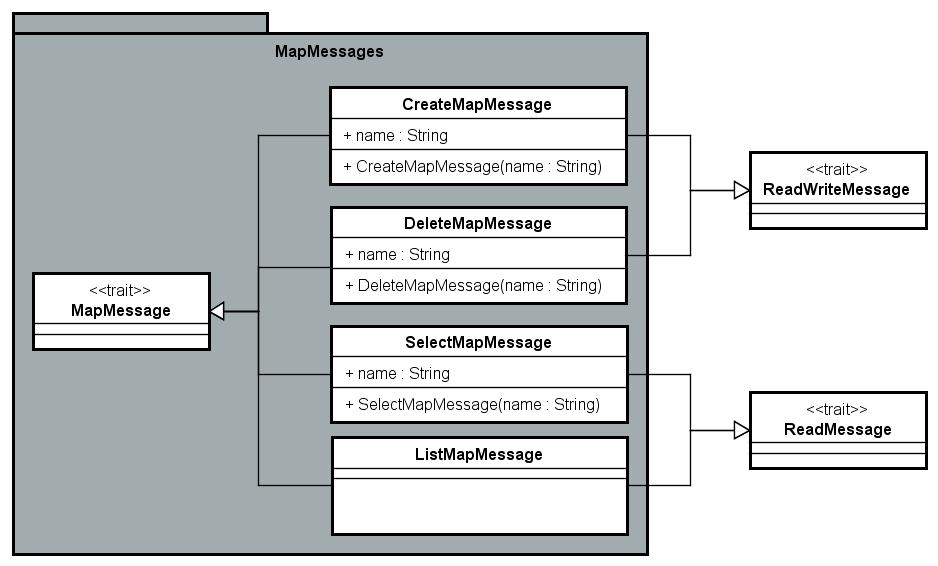
\includegraphics[width=\textwidth]{ST/Server/mapMessagesLevel.jpg}
				\caption{Componente Actorbase.server.messages.query.user.MapMessages}
			\end{figure}
			
			\subsubsection{Descrizione}
				Pacchetto contenente i messaggi che rappresentano le query a livello di mappa.				
				
			\subsubsection{Classi}
				\begin{itemize}
					\item Actorbase.server.messages.query.user.MapMessages.CreateMapMessage
					\item Actorbase.server.messages.query.user.MapMessages.DeleteMapMessage
					\item Actorbase.server.messages.query.user.MapMessages.SelectMapMessage
					\item Actorbase.server.messages.query.user.MapMessages.ListMapMessage
				\end{itemize}
				
			\subsubsection{Trait}
				\begin{itemize}
					\item Actorbase.server.messages.query.user.MapMessages.MapMessage
				\end{itemize}
		
		\subsection{Actorbase.server.messages.query.user.MapMessages.MapMessage}
			\subsubsection{Descrizione}
				Trait che rappresenta i messaggi contenenti richieste a livello di mappa.
				
			\subsubsection{Utilizzo}
				Viene utilizzato per poter riconoscere i messaggi contenenti richieste a livello di mappa.
				
			\subsubsection{Relazioni con altre classi}
				\begin{itemize}
					\item \textbf{Actorbase.server.utils.Parser:} relazione entrante di creazione.
					\item \textbf{Actorbase.server.actors.Usermanager:} relazione di utilizzo.
					\item \textbf{Actorbase.server.actors.Main:} relazione di utilizzo.
					\item \textbf{Actorbase.server.actors.Storemanager:} relazione di utilizzo.
					\item \textbf{Actorbase.server.actors.Storefinder:} relazione di utilizzo.
					\item \textbf{Actorbase.server.actors.Warehouseman:} relazione di utilizzo.
				\end{itemize}
				
			\subsubsection{Classi figlie}
				\begin{itemize}
					\item Actorbase.server.messages.query.user.MapMessages.CreateMapMessage
					\item Actorbase.server.messages.query.user.MapMessages.DeleteMapMessage
					\item Actorbase.server.messages.query.user.MapMessages.SelectMapMessage
					\item Actorbase.server.messages.query.user.MapMessages.ListMapMessage
				\end{itemize}
				
		\subsection{Actorbase.server.messages.query.user.MapMessages.CreateMapMessage}
			\subsubsection{Descrizione}
				Classe che rappresenta un messaggio contente la richiesta di creazione di una mappa in un database.
				
			\subsubsection{Utilizzo}
				Effettua il percorso descritto in \hyperref[QueryMessage]{Actorbase.server.messages.query.QueryMessage} saltando l'attore \textbf{Storekeeper}.
				
			\subsubsection{Relazioni con altre classi}
				\begin{itemize}
					\item \textbf{Actorbase.server.utils.Parser:} relazione entrante di creazione.
					\item \textbf{Actorbase.server.actors.Usermanager:} relazione di utilizzo.
					\item \textbf{Actorbase.server.actors.Main:} relazione di utilizzo.
					\item \textbf{Actorbase.server.actors.Storemanager:} relazione di utilizzo.
					\item \textbf{Actorbase.server.actors.Storefinder:} relazione di utilizzo.
					\item \textbf{Actorbase.server.actors.Warehouseman:} relazione di utilizzo.
				\end{itemize}
			\subsubsection{Trait implementati}
				\begin{itemize}
					\item Actorbase.server.messages.query.user.MapMessages.MapMessage
				\end{itemize}
				
		\subsection{Actorbase.server.messages.query.user.MapMessages.DeleteMapMessage}
			\subsubsection{Descrizione}
				Classe che rappresenta un messaggio contente la richiesta di rimozione di una mappa in un database.
				
			\subsubsection{Utilizzo}
				Effettua il percorso descritto in \hyperref[QueryMessage]{Actorbase.server.messages.query.QueryMessage} saltando l'attore \textbf{Storekeeper}.
				
			\subsubsection{Relazioni con altre classi}
				\begin{itemize}
					\item \textbf{Actorbase.server.utils.Parser:} relazione entrante di creazione.
					\item \textbf{Actorbase.server.actors.Usermanager:} relazione di utilizzo.
					\item \textbf{Actorbase.server.actors.Main:} relazione di utilizzo.
					\item \textbf{Actorbase.server.actors.Storemanager:} relazione di utilizzo.
					\item \textbf{Actorbase.server.actors.Storefinder:} relazione di utilizzo.
					\item \textbf{Actorbase.server.actors.Warehouseman:} relazione di utilizzo.
				\end{itemize}
			\subsubsection{Trait implementati}
				\begin{itemize}
					\item Actorbase.server.messages.query.user.MapMessages.MapMessage
				\end{itemize}
				
		\subsection{Actorbase.server.messages.query.user.MapMessages.SelectMapMessage}
			\subsubsection{Descrizione}
				Classe che rappresenta un messaggio contente la richiesta di selezione di una mappa in un database.
				
			\subsubsection{Utilizzo}
				Effettua il percorso descritto in \hyperref[QueryMessage]{Actorbase.server.messages.query.QueryMessage} saltando l'attore \textbf{Storekeeper}.
				
			\subsubsection{Relazioni con altre classi}
				\begin{itemize}
					\item \textbf{Actorbase.server.utils.Parser:} relazione entrante di creazione.
					\item \textbf{Actorbase.server.actors.Usermanager:} relazione di utilizzo.
					\item \textbf{Actorbase.server.actors.Main:} relazione di utilizzo.
					\item \textbf{Actorbase.server.actors.Storemanager:} relazione di utilizzo.
					\item \textbf{Actorbase.server.actors.Storefinder:} relazione di utilizzo.
					\item \textbf{Actorbase.server.actors.Warehouseman:} relazione di utilizzo.
				\end{itemize}
			\subsubsection{Trait implementati}
				\begin{itemize}
					\item Actorbase.server.messages.query.user.MapMessages.MapMessage
				\end{itemize}
				
		\subsection{Actorbase.server.messages.query.user.MapMessages.ListMapMessage}
			\subsubsection{Descrizione}
				Classe che rappresenta un messaggio contente la richiesta di visualizzazione di tutte le mappe presenti in un database.
				
			\subsubsection{Utilizzo}
				Effettua il percorso descritto in \hyperref[QueryMessage]{Actorbase.server.messages.query.QueryMessage} saltando l'attore \textbf{Storekeeper}.
				
			\subsubsection{Relazioni con altre classi}
				\begin{itemize}
					\item \textbf{Actorbase.server.utils.Parser:} relazione entrante di creazione.
					\item \textbf{Actorbase.server.actors.Usermanager:} relazione di utilizzo.
					\item \textbf{Actorbase.server.actors.Main:} relazione di utilizzo.
					\item \textbf{Actorbase.server.actors.Storemanager:} relazione di utilizzo.
					\item \textbf{Actorbase.server.actors.Storefinder:} relazione di utilizzo.
					\item \textbf{Actorbase.server.actors.Warehouseman:} relazione di utilizzo.
				\end{itemize}
			\subsubsection{Trait implementati}
				\begin{itemize}
					\item Actorbase.server.messages.query.user.MapMessages.MapMessage
				\end{itemize}
				
		\subsection{Actorbase.server.messages.query.user.DatabaseMessages}
		
			\begin{figure}[H]
				\centering
				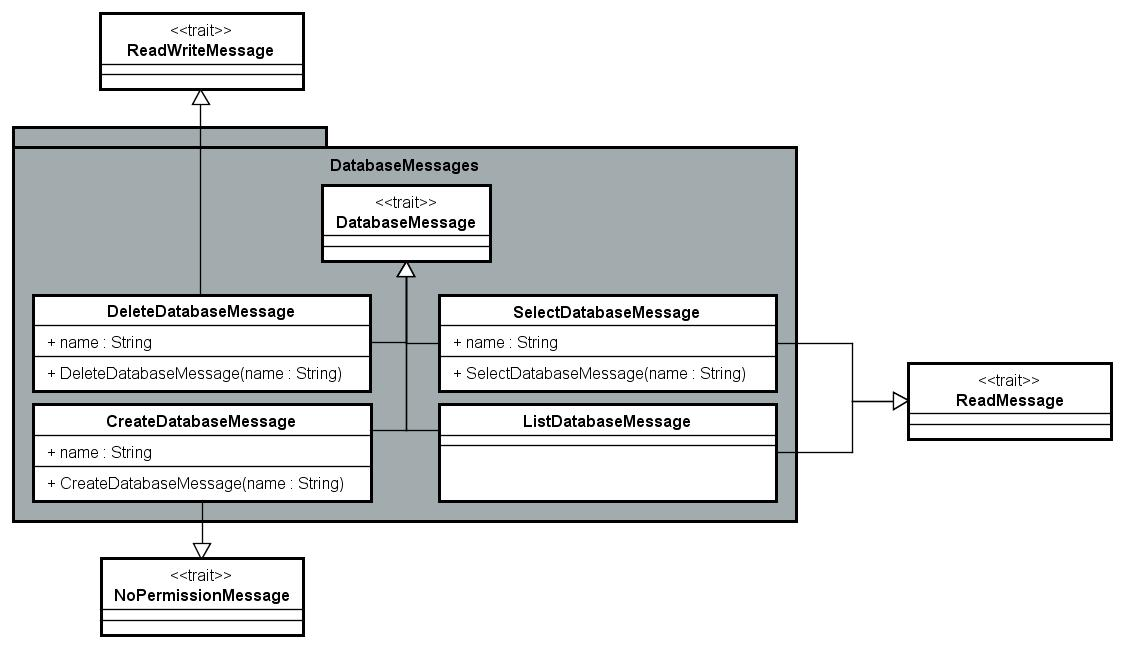
\includegraphics[width=\textwidth]{ST/Server/databaseMessagesLevel.jpg}
				\caption{Componente Actorbase.server.messages.query.user.DatabaseMessages}
			\end{figure}
			
			\subsubsection{Descrizione}
				Pacchetto contenente i messaggi che rappresentano le query a livello di database.				
				
			\subsubsection{Classi}
				\begin{itemize}
					\item Actorbase.server.messages.query.user.DatabaseMessages.CreateDatabaseMessage
					\item Actorbase.server.messages.query.user.DatabaseMessages.DeleteDatabaseMessage
					\item Actorbase.server.messages.query.user.DatabaseMessages.SelectDatabaseMessage
					\item Actorbase.server.messages.query.user.DatabaseMessages.ListDatabaseMessage
				\end{itemize}
				
			\subsubsection{Trait}
				\begin{itemize}
					\item Actorbase.server.messages.query.user.DatabaseMessages.DatabaseMessage
				\end{itemize}
				
		\subsection{Actorbase.server.messages.query.user.DatabaseMessages.DatabaseMessage}
			\subsubsection{Descrizione}
				Trait che rappresenta i messaggi contenenti richieste a livello di database.
				
			\subsubsection{Utilizzo}
				Viene utilizzato per poter distinguere i messaggi contenenti richieste a livello di database.
				
			\subsubsection{Relazioni con altre classi}
				\begin{itemize}
					\item \textbf{Actorbase.server.utils.Parser:} relazione entrante di creazione.
					\item \textbf{Actorbase.server.actors.Usermanager:} relazione di utilizzo.
					\item \textbf{Actorbase.server.actors.Main:} relazione di utilizzo.
					\item \textbf{Actorbase.server.actors.Warehouseman:} relazione di utilizzo.
				\end{itemize}
			\subsubsection{Classi figlie}
				\begin{itemize}
					\item Actorbase.server.messages.query.user.DatabaseMessages.CreateDatabaseMessage
					\item Actorbase.server.messages.query.user.DatabaseMessages.DeleteDatabaseMessage
					\item Actorbase.server.messages.query.user.DatabaseMessages.SelectDatabaseMessage
					\item Actorbase.server.messages.query.user.DatabaseMessages.ListDatabaseMessage
				\end{itemize}
		
		\subsection{Actorbase.server.messages.query.user.DatabaseMessages.CreateDatabaseMessage}
			\subsubsection{Descrizione}
				Classe che rappresenta un messaggio contenente la richiesta di creazione di un database.
				
			\subsubsection{Utilizzo}
				Effettua il percorso descritto in \hyperref[QueryMessage]{Actorbase.server.messages.query.QueryMessage} fermandosi all'attore \textbf{Main}.
				Viene inoltre inoltrato ai \textbf{Warehouseman}.
				
			\subsubsection{Relazioni con altre classi}
				\begin{itemize}
					\item \textbf{Actorbase.server.utils.Parser:} relazione entrante di creazione.
					\item \textbf{Actorbase.server.actors.Usermanager:} relazione di utilizzo.
					\item \textbf{Actorbase.server.actors.Main:} relazione di utilizzo.
					\item \textbf{Actorbase.server.actors.Warehouseman:} relazione di utilizzo.
				\end{itemize}
			\subsubsection{Trait implementati}
				\begin{itemize}
					\item Actorbase.server.messages.query.user.DatabaseMessages.DatabaseMessage
				\end{itemize}
				
		\subsection{Actorbase.server.messages.query.user.DatabaseMessages.DeleteDatabaseMessage}
			\subsubsection{Descrizione}
				Classe che rappresenta un messaggio contenente la richiesta di rimozione di un database.
				
			\subsubsection{Utilizzo}
				Effettua il percorso descritto in \hyperref[QueryMessage]{Actorbase.server.messages.query.QueryMessage} fermandosi all'attore \textbf{Main}.
				Viene inoltre inoltrato ai \textbf{Warehouseman}.
				
			\subsubsection{Relazioni con altre classi}
				\begin{itemize}
					\item \textbf{Actorbase.server.utils.Parser:} relazione entrante di creazione.
					\item \textbf{Actorbase.server.actors.Usermanager:} relazione di utilizzo.
					\item \textbf{Actorbase.server.actors.Main:} relazione di utilizzo.
					\item \textbf{Actorbase.server.actors.Warehouseman:} relazione di utilizzo.
				\end{itemize}
			\subsubsection{Trait implementati}
				\begin{itemize}
					\item Actorbase.server.messages.query.user.DatabaseMessages.DatabaseMessage
				\end{itemize}
				
		\subsection{Actorbase.server.messages.query.user.DatabaseMessages.SelectDatabaseMessage}
			\subsubsection{Descrizione}
				Classe che rappresenta un messaggio contenente la richiesta di selezione di un database.
				
			\subsubsection{Utilizzo}
				Effettua il percorso descritto in \hyperref[QueryMessage]{Actorbase.server.messages.query.QueryMessage} fermandosi all'attore \textbf{Main}.
				Viene inoltre inoltrato ai \textbf{Warehouseman}.
				
			\subsubsection{Relazioni con altre classi}
				\begin{itemize}
					\item \textbf{Actorbase.server.utils.Parser:} relazione entrante di creazione.
					\item \textbf{Actorbase.server.actors.Usermanager:} relazione di utilizzo.
					\item \textbf{Actorbase.server.actors.Main:} relazione di utilizzo.
					\item \textbf{Actorbase.server.actors.Warehouseman:} relazione di utilizzo.
				\end{itemize}
			\subsubsection{Trait implementati}
				\begin{itemize}
					\item Actorbase.server.messages.query.user.DatabaseMessages.DatabaseMessage
				\end{itemize}
				
		\subsection{Actorbase.server.messages.query.user.DatabaseMessages.ListDatabaseMessage}
			\subsubsection{Descrizione}
				Classe che rappresenta un messaggio contenente la richiesta di visualizzazione dell'intera lista di database presenti.
				
			\subsubsection{Utilizzo}
				Effettua il percorso descritto in \hyperref[QueryMessage]{Actorbase.server.messages.query.QueryMessage} fermandosi all'attore \textbf{Main}.
				
			\subsubsection{Relazioni con altre classi}
				\begin{itemize}
					\item \textbf{Actorbase.server.utils.Parser:} relazione entrante di creazione.
					\item \textbf{Actorbase.server.actors.Usermanager:} relazione di utilizzo.
					\item \textbf{Actorbase.server.actors.Main:} relazione di utilizzo.
					\item \textbf{Actorbase.server.actors.Warehouseman:} relazione di utilizzo.
				\end{itemize}
			\subsubsection{Trait implementati}
				\begin{itemize}
					\item Actorbase.server.messages.query.user.DatabaseMessages.DatabaseMessage
				\end{itemize}
				
		\subsection{Actorbase.server.messages.query.user.HelpMessages}
		
			\begin{figure}[H]
				\centering
				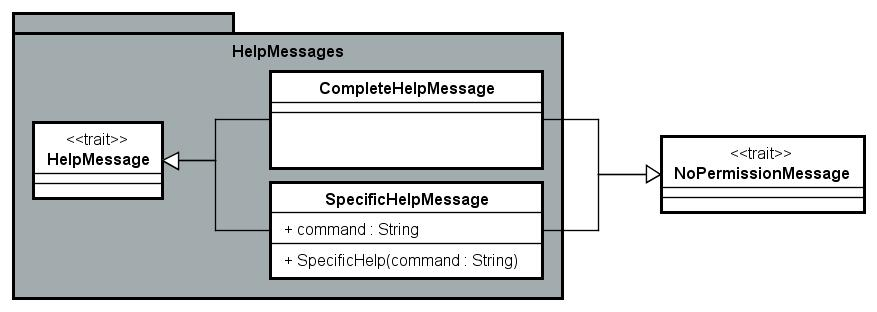
\includegraphics[width=\textwidth]{ST/Server/helpMessagesLevel.jpg}
				\caption{Componente Actorbase.server.messages.query.user.HelpMessages}
			\end{figure}
			
			\subsubsection{Descrizione}
				Pacchetto contenente i messaggi che rappresentano le query di aiuto.				
				
			\subsubsection{Classi}
				\begin{itemize}
					\item Actorbase.server.messages.query.user.HelpMessages.CompleteHelp
					\item Actorbase.server.messages.query.user.HelpMessages.SpecificHelp
				\end{itemize}
				
			\subsubsection{Trait}
				\begin{itemize}
					\item Actorbase.server.messages.query.user.HelpMessages.HelpMessage
				\end{itemize}
		
		\subsection{Actorbase.server.messages.query.user.HelpMessages.HelpMessage}
			\subsubsection{Descrizione}
				Trait che rappresenta i messaggi contenenti richieste per la visualizzazione di aiuti.
				
			\subsubsection{Utilizzo}
				Viene utilizzata per poter distinguere i messaggi contenenti richieste per la visualizzazione di aiuti.
			\subsubsection{Relazioni con altre classi}
				\begin{itemize}
					\item \textbf{Actorbase.server.utils.Parser:} relazione entrante di creazione.
					\item \textbf{Actorbase.server.actors.Usermanager:} relazione di utilizzo.
					\item \textbf{Actorbase.server.actors.Main:} relazione di utilizzo.
				\end{itemize}
			\subsubsection{Classi figlie}
				\begin{itemize}
					\item Actorbase.server.messages.query.user.HelpMessages.CompleteHelp
					\item Actorbase.server.messages.query.user.HelpMessages.SpecificHelp
				\end{itemize}
		
		\subsection{Actorbase.server.messages.query.user.HelpMessages.CompleteHelp}
			\subsubsection{Descrizione}
				Classe che rappresenta i messaggi contenenti richieste per la visualizzazione di tutti i comandi disponibili.
				
			\subsubsection{Utilizzo}
				Effettua il percorso descritto in \hyperref[QueryMessage]{Actorbase.server.messages.query.QueryMessage} fermandosi all'attore \textbf{Main}.
				
			\subsubsection{Relazioni con altre classi}
				\begin{itemize}
					\item \textbf{Actorbase.server.utils.Parser:} relazione entrante di creazione.
					\item \textbf{Actorbase.server.actors.Usermanager:} relazione di utilizzo.
					\item \textbf{Actorbase.server.actors.Main:} relazione di utilizzo.
				\end{itemize}
			\subsubsection{Trait implementati}
				\begin{itemize}
					\item Actorbase.server.messages.query.user.HelpMessages.HelpMessage
				\end{itemize}

		\subsection{Actorbase.server.messages.query.user.HelpMessages.SpecificHelp}
			\subsubsection{Descrizione}
				Classe che rappresenta i messaggi contenenti richieste per la visualizzazione di aiuto riguardante un comando specifico.
				
			\subsubsection{Utilizzo}
				Effettua il percorso descritto in \hyperref[QueryMessage]{Actorbase.server.messages.query.QueryMessage} fermandosi all'attore \textbf{Main}.
				
			\subsubsection{Relazioni con altre classi}
				\begin{itemize}
					\item \textbf{Actorbase.server.utils.Parser:} relazione entrante di creazione.
					\item \textbf{Actorbase.server.actors.Usermanager:} relazione di utilizzo.
					\item \textbf{Actorbase.server.actors.Main:} relazione di utilizzo.
				\end{itemize}
			\subsubsection{Trait implementati}
				\begin{itemize}
					\item Actorbase.server.messages.query.user.HelpMessages.HelpMessage
				\end{itemize}
			
		\subsection{Actorbase.client}
		
			\begin{figure}[H]
				\centering
				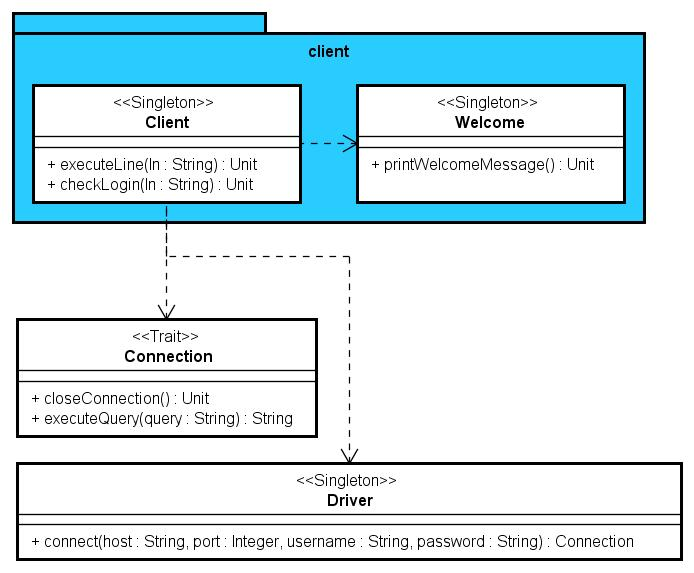
\includegraphics[width=\textwidth]{ST/Client/clientLevel.jpg}
				\caption{Componente Actorbase.client}
			\end{figure}
			\subsubsection{Descrizione}
				Package per la componente lato client del sistema. 
				È composto due classi che implementano il design pattern \textbf{Singleton}.
				
			\subsubsection{Classi}
				\begin{itemize}
					\item Actorbase.client.Client
					\item Actorbase.client.Welcome
				\end{itemize}
				
		\subsection{Actorbase.client.Client}
			\subsubsection{Descrizione}
				Questa classe fornisce un'interfaccia a linea di comando e permette all'utente di inserire i comandi che verranno inviati al server. 
				Questa classe implementa il design pattern \textbf{Singleton}.
				
			\subsubsection{Utilizzo}
				Viene utilizzata per distinguere i comandi di connessione, disconnessione e altri comandi possibili. Inoltre utilizza il driver per comunicare 
				con il server.
				
			\subsubsection{Relazioni con altre classi}
				\begin{itemize}
					\item \textbf{Actorbase.client.Welcome:} relazione di utilizzo.
					\item \textbf{Actorbase.driver.Driver:} relazione di utilizzo.
					\item \textbf{Actorbase.driver.Connection:} relazione di utilizzo.
				\end{itemize}
		
		\subsection{Actorbase.client.Welcome}
			\subsubsection{Descrizione}
				Classe si supporto per stampare un messaggio di benvenuto sulla console del client.
				
			\subsubsection{Utilizzo}
				Viene utilizzata dal client per stampare un messaggio di benvenuto all'avvio dell'interfaccia a linea di comando.
				
			\subsubsection{Relazioni con altre classi}
				\begin{itemize}
					\item \textbf{Actorbase.client.Client}
				\end{itemize}
				
		\subsection{Actorbase.driver}
		
			\begin{figure}[H]
				\centering
				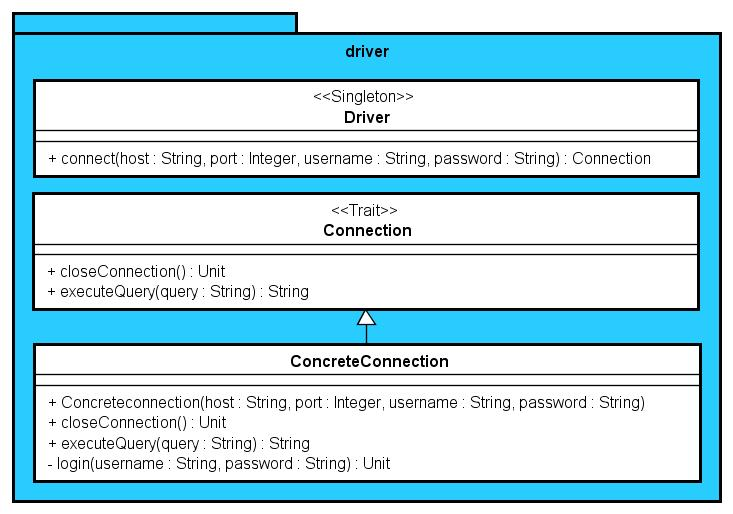
\includegraphics[width=\textwidth]{ST/Driver/driverLevel.jpg}
				\caption{Componente Actorbase.driver}
			\end{figure}
			\subsubsection{Descrizione}
				Package per la componente driver del sistema. 
				È composto una classe che implementa il design pattern \textbf{Singleton}, un trait e una sua implementazione.
				
			\subsubsection{Classi}
				\begin{itemize}
					\item Actorbase.driver.Driver
					\item Actorbase.driver.ConcreteConnection
				\end{itemize}
			
			\subsubsection{Trait}
				\begin{itemize}
					\item Actorbase.driver.Connection
				\end{itemize}
					
		\subsection{Actorbase.driver.Connection}
			\subsubsection{Descrizione}
				Trait utilizzato per effettuare il login su un determinato server.
				 
			\subsubsection{Utilizzo}
				Costruisce una query nel modo corretto ricevendo un comando in formato stringa dal client.
				
			\subsubsection{Relazioni con altre classi}
				\begin{itemize}
					\item \textbf{Actorbase.driver.Driver:} relazione entrante, creazione.
					\item \textbf{Actorbase.driver.Client:} relazione di utilizzo.
				\end{itemize}
			\subsubsection{Classi figlie}
				\begin{itemize}
					\item Actorbase.driver.ConcreteConnection
				\end{itemize}
				
		\subsection{Actorbase.driver.ConcreteConnection}
			\subsubsection{Descrizione}
				Classe utilizzata per effettuare il login su un determinato server. Apre una connessione verso il server specificato.
				
			\subsubsection{Utilizzo}
				Costruisce una query nel modo corretto ricevendo un comando in formato stringa dal client.
				
			\subsubsection{Relazioni con altre classi}
				\begin{itemize}
					\item \textbf{Actorbase.driver.Driver:} relazione entrante, creazione.
					\item \textbf{Actorbase.driver.Client:} relazione di utilizzo.
				\end{itemize}
			\subsubsection{Trait implementati}
				\begin{itemize}
					\item Actorbase.driver.Connection
				\end{itemize}
				
		\subsection{Actorbase.driver.Driver}
			\subsubsection{Descrizione}
				Classe che implementa il design pattern \textbf{Singleton}, 
				
			\subsubsection{Utilizzo}
				Viene utilizzato per creare una connessione che viene restituita al client. 
				
			\subsubsection{Relazioni con altre classi}
				\begin{itemize}
					\item \textbf{Actorbase.client.Client:} relazione di utilizzo.
					\item \textbf{Actorbase.driver.ConcreteConnection:} relazione uscente, creazione.
				\end{itemize}
		
		
		%%%%%%%%%%% OLD
	\newpage 
	\section{Diagrammi delle attività}
		Segue il diagramma delle attività che mostra l'interazione dell'utente con il client.
		\subsubsection{Diagramma attività principale}
		
		\begin{figure} [H]
			\centering
			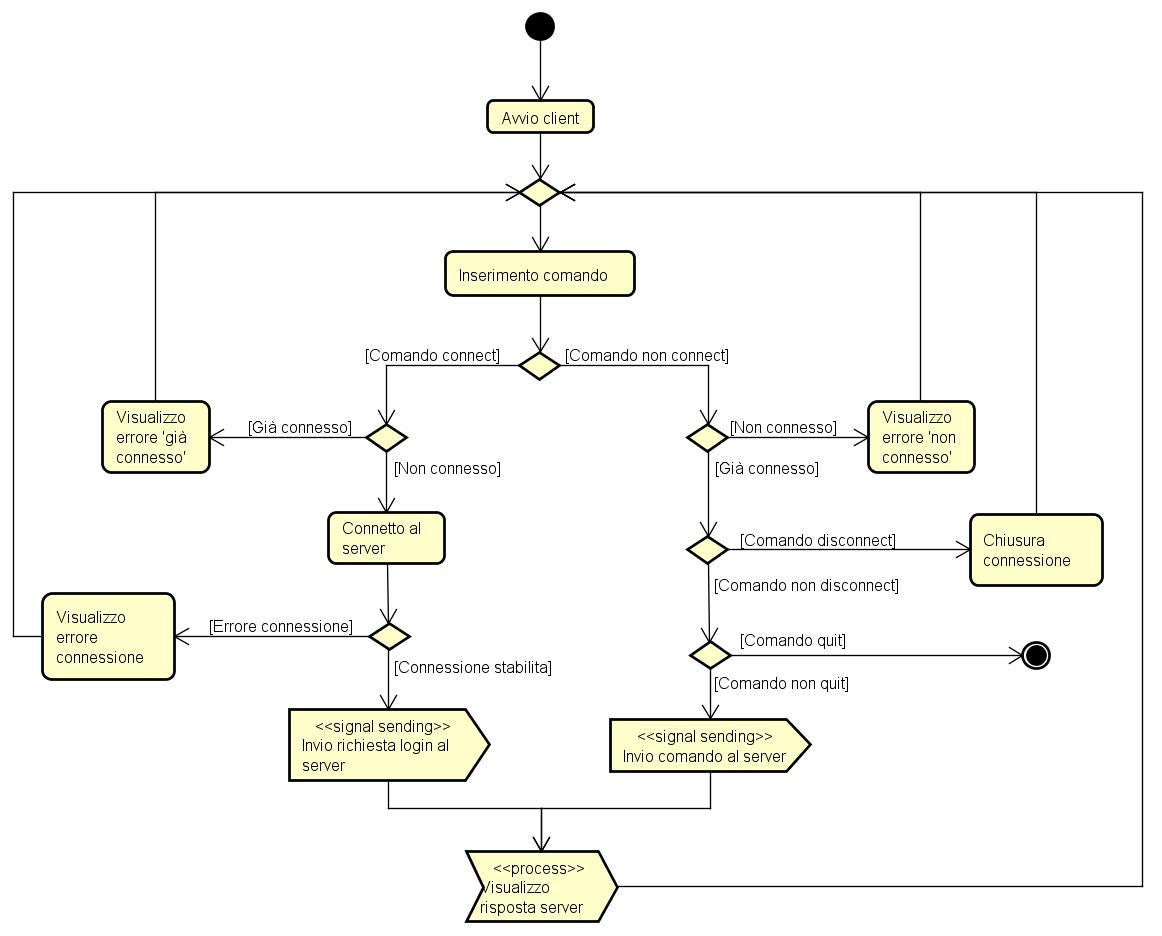
\includegraphics[width=\textwidth]{ST/Attivita/attivitaPrincipale.jpg}
			\caption{Diagramma attività principale}
		\end{figure}
		Dopo aver avviato il client l'utente può inserire dei comandi. Se il comando è di chiusura il client si spegne. Se il comando è di connect ed il client non è connesso quest'ultimo si connette ed invia un comando di login al server, altrimenti stampa un messaggio di errore. Se il comando non è di connect ed il client è connesso quest'ultimo lo controlla. Se esso è un comando di disconnessione il client si disconnette dal server, altrimenti invia la richiesta.
		
	\newpage 
	\section{Diagrammi di sequenza}
        In questa sezione verranno illustrati e descritti i principali diagrammi di sequenza realizzati. Questi ultimi illustrano le azioni compiute dal server per l'avvio e la gestire le richieste utente.
        
        Per esplicitare l'invio di un messaggio tra due attori, nei diagrammi viene chiamato il metodo \textit{receive()} dell'attore che riceve il messaggio 
        da parte di chi lo invia.
        Questo è dovuto al fatto che tutte le classi ereditano dall'interfaccia \textit{Actor} messa a disposizione da \textit{Akka} senza effettuare 
        l'override del metodo per inviare i messaggi; mentre sovrascrivono il metodo di ricezione per gestire i messaggi in entrata.
        
        Trattandosi di diagrammi di sequenza non molto specifici, alcuni attori effettuano operazioni senza chiamare dei metodi specifici già 
        dichiarati. 
       \subsection{Avvio}
            \begin{figure} [H]
				\centering
				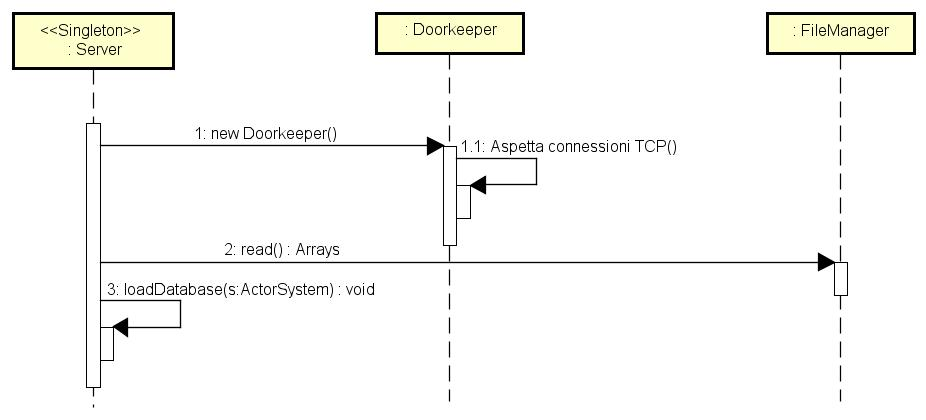
\includegraphics[width=\textwidth]{ST/Sequenza/seqAvvio.jpg}
				\caption{Diagramma di sequenza - avvio del server.}
			\end{figure}
            Nel diagramma precedente è possibile visualizzare quali sono le operazioni che vengono eseguite per avviare il server. Esso crea i vari Doorkeeper, i punti di accesso dall'esterno, che resteranno in ascolto di connessioni in entrata. Poi legge le configurazioni salvate su disco e carica i database.
             
       \subsection{Nuova connessione}
            \begin{figure} [H]
				\centering
				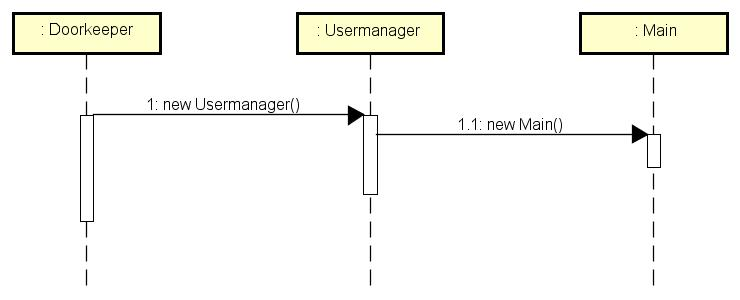
\includegraphics[width=\textwidth]{ST/Sequenza/seqNuovaConnessione.jpg}
				\caption{Diagramma di sequenza - nuova connessione al server.}
			\end{figure}
            Nel diagramma precedente è possibile visualizzare quali sono le operazioni che vengono eseguite quando un client si collega al socket TCP di un Doorkeeper. Per ogni nuova connessione l'attore Doorkeeper crea un attore Usermanager il quale crea un attore Main. Usermanager gestisce ogni richiesta proveniente dalla connessione a lui associata, nello specifico trasforma i comandi in forma testuale in messaggi da inoltrare al Main.
            
        \subsection{Comando utente}
            \begin{figure} [H]
				\centering
				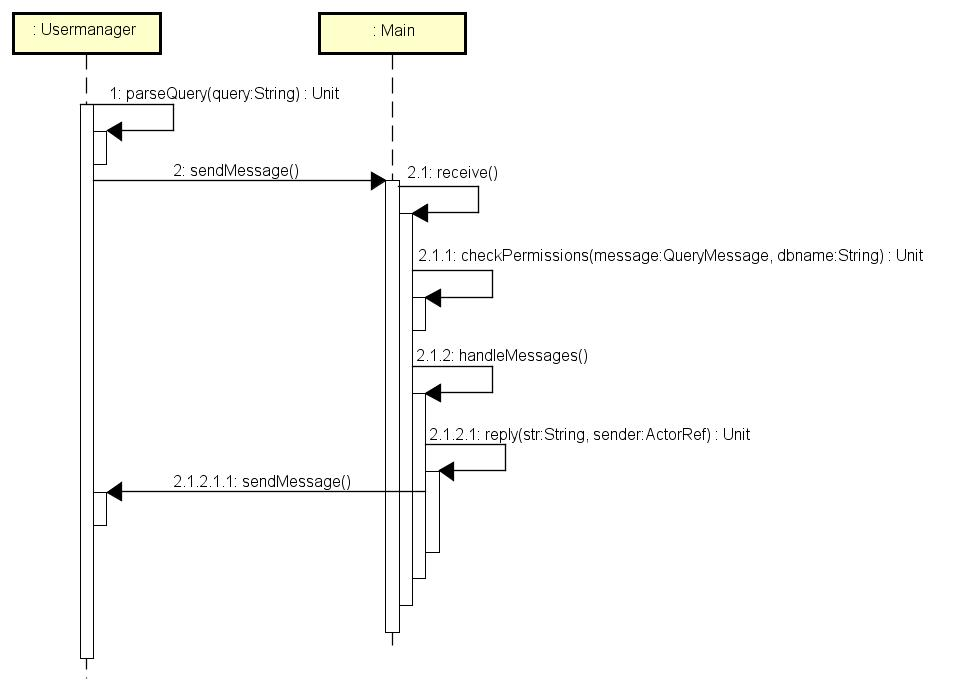
\includegraphics[width=\textwidth]{ST/Sequenza/seqComandoUtente.jpg}
				\caption{Diagramma di sequenza - gestione comando utente.}
			\end{figure}
            Nel diagramma precedente è possibile visualizzare quali sono le operazioni che vengono eseguite dagli attori Usermanager e Main alla ricezione di una richiesta dall'utente. 
Usermanager, dopo aver convertito i byte ricevuti in una stringa, crea un messaggio che rappresenta la richiesta dell'utente ed lo invia al Main. Il Main controlla che l'utente abbia i permessi per il tipo di richiesta, in caso affermativo gestisce, anche indirettamente, il messaggio e risponde.             
            
        \subsection{Richiesta di creazione mappa}
            \begin{figure} [H]
				\centering
				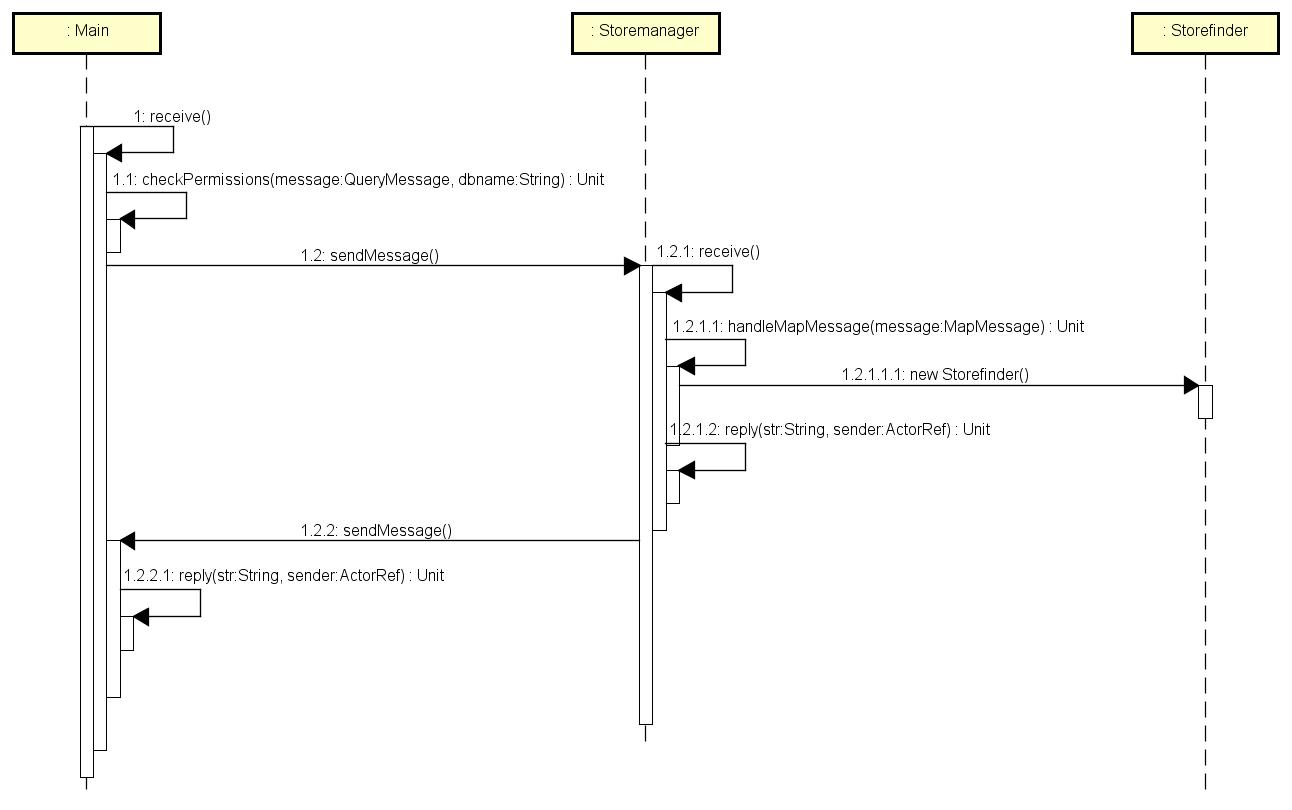
\includegraphics[width=\textwidth]{ST/Sequenza/seqNuovaMappa.jpg}
				\caption{Diagramma di sequenza - gestione di richiesta di creazione mappa.}
			\end{figure}
            Nel diagramma precedente è possibile visualizzare quali sono le operazioni che vengono eseguite quando il Main riceve una richiesta di creazione di una mappa. Il Main alla ricezione di un messaggio, dopo aver controllato i permessi, ne controlla il tipo. Se è un messaggio di tipo mappa lo inoltra allo Storemanager che rappresenta il database precedentemente selezionato. Lo Storemanager crea un nuovo Storefinder che rappresenterà la mappa e risponde con l'esito che arriverà fino al client.
            
        \subsection{Richiesta di find}
            \begin{figure} [H]
				\centering
				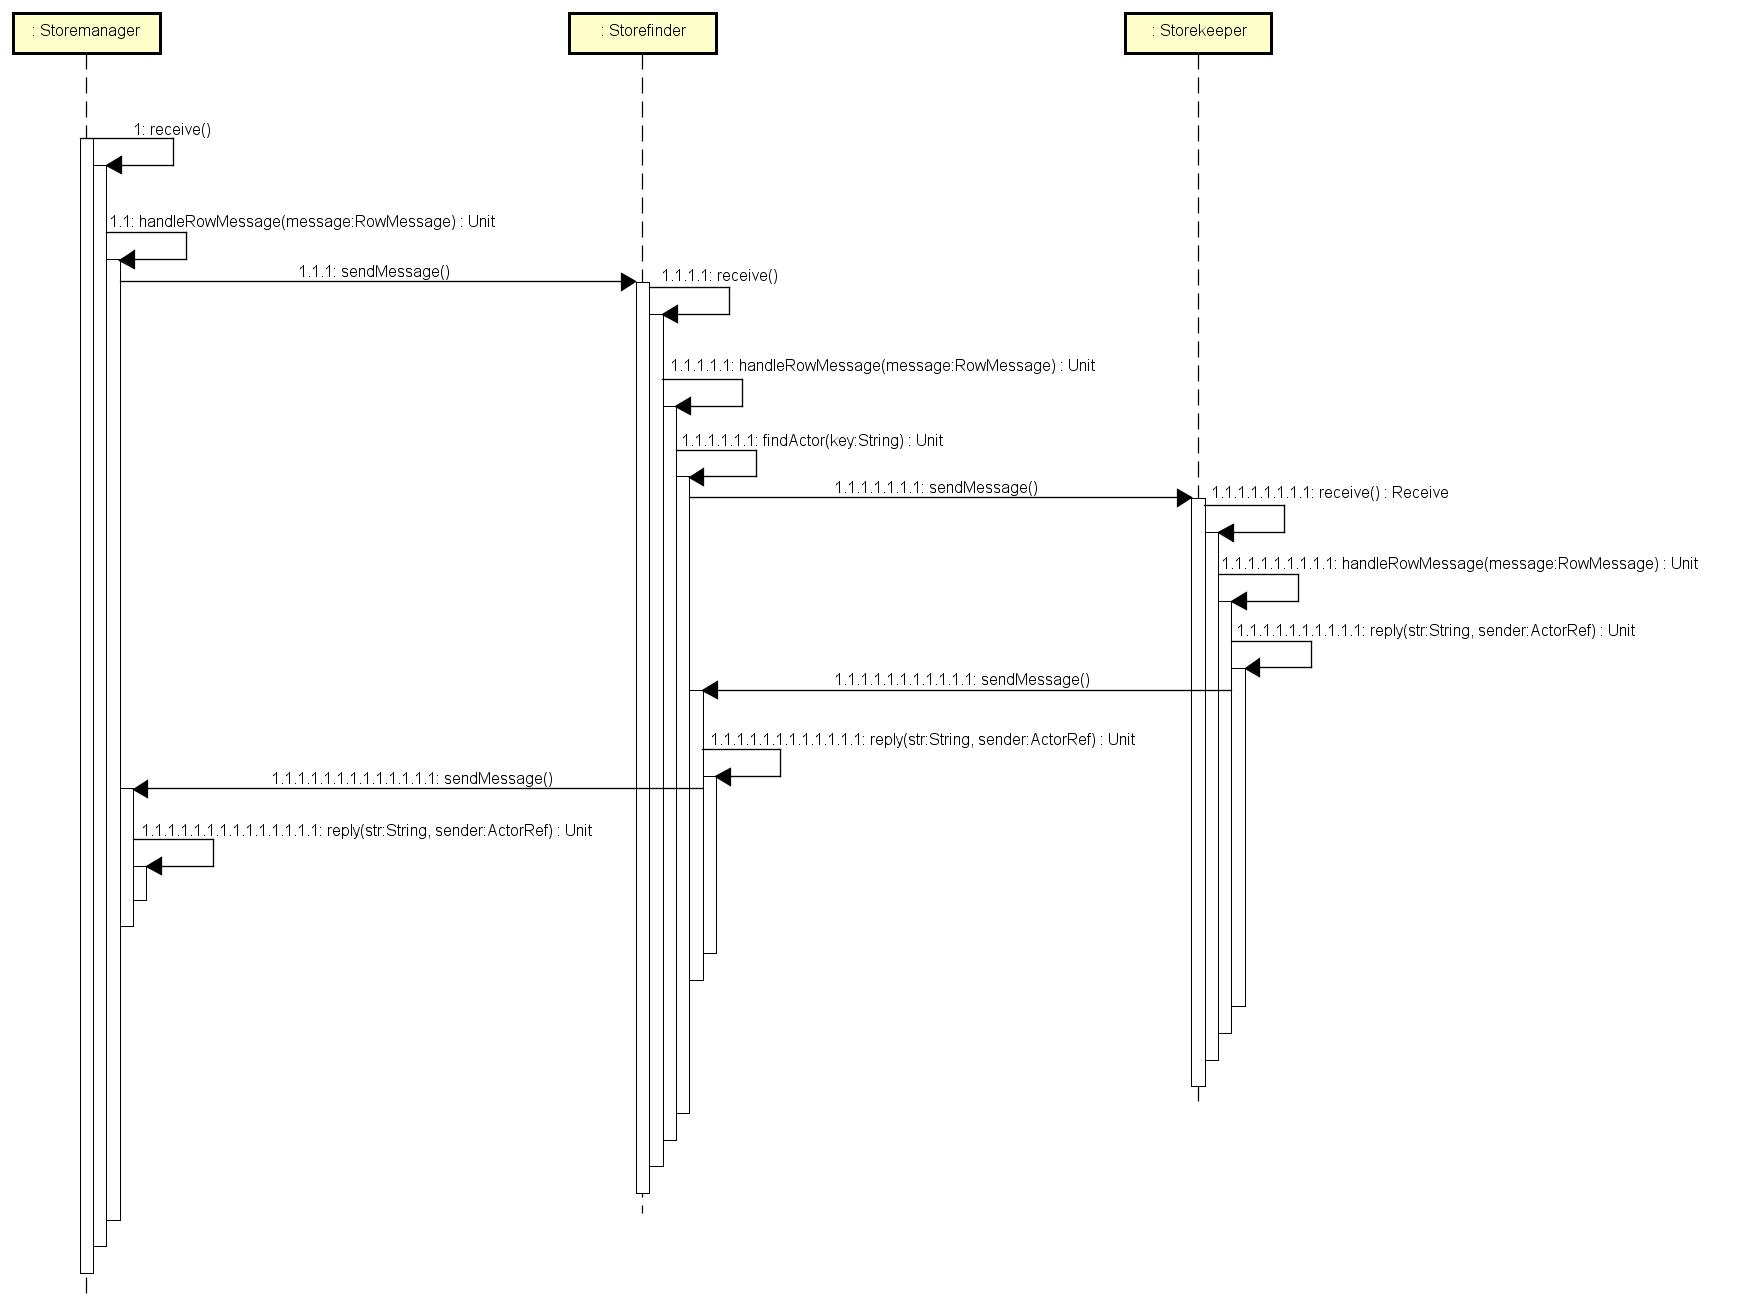
\includegraphics[width=\textwidth]{ST/Sequenza/seqFind.jpg}
				\caption{Diagramma di sequenza - gestione di richiesta di Find.}
			\end{figure}
            Nel diagramma precedente è possibile visualizzare quali sono le operazioni che vengono eseguite per gestire una richiesta di find. Il messaggio rappresentante un comando find viene inoltrato fino allo Storekeeper responsabile dell'area di mappa richiesta. Lo Storekeeper risponderà con il valore delle chiave o con un messaggio di errore. La risposta verrà poi inoltrata all'indietro fino al client.            
	\section{Desing Pattern utilizzati}
	Segue la descrizione delle parti dell'architettura che utilizzano desing pattern. I desing pattern sono descritti in appendice.
	\subsection{Broker event-driven}
	Il sistema ad attori di Akka è molto simile ad un architettura event-driven di tipologia broker, di conseguenza il server di Actorbase segue questa architettura, nella quale gli attori svolgono il ruolo di Event Processor mentre l'Actor System crea i suddetti attori e svolge anche la funzione di Event Channel.
	\subsection{Singleton}
	Le classi Server e Client seguono il desing pattern Singleton, realizzato definendo le classi come Object, cosi facendo Scala garantisce che ci sia una solo istanza di queste classi per ogni esecuzione del programma.        
	\newpage 
	\section{Stime di fattibilità e di bisogno di risorse}
	
		L'architettura definita fino a questo punto è sufficiente per fornire una stima della fattibilità del prodotto e delle risorse richieste per la realizzazione. \\
	Il gruppo inizialmente non aveva conoscenze sufficienti per stimare in modo appropriato la complessità dell'implementazione di un Database basato sulla logica ad attori. Grazie al livello di dettaglio raggiunto sono stati fugati molti dei dubbi e delle incertezze a riguardo, confermando le previsioni sull'esito positivo del progetto. \\
	Sono state inoltre individuate con chiarezza le risorse tecnologiche che verranno utilizzate:
	\begin{itemize}
		\item Akka: libreria per modello ad attori.
		\item IntelliJ: framework per la stesura del codice.
		\item JVM: piattaforma per il funzionamento di Scala.
	\end{itemize}
	Il gruppo in contemporanea si è dedicato allo studio delle nuove tecnologie raggiungendo un buon livello di conoscenza. L'insieme di queste risorse potrà garantire la realizzazione di tutte le componenti dell'architettura.
	
	\newpage 
	\section{Tracciamento}
		\subsection{Tracciamento componenti-requisiti}
			\LTXtable{\textwidth}{Tabelle/tabelle_componenti_requisiti/componenti_requisiti.tex}
		\subsection{Tracciamento requisiti-componenti}
			\LTXtable{\textwidth}{Tabelle/tabelle_componenti_requisiti/requisiti_componenti.tex}
		
	\newpage 
	\section{Appendice}
	\subsection{Descrizione Design Pattern}
	Segue, per ogni Design Pattern utilizzato, la descrizione dello scopo, motivazione e applicabilità.
	\subsubsection{Broker event-driven}
				\begin{figure}[H]
					\centering
					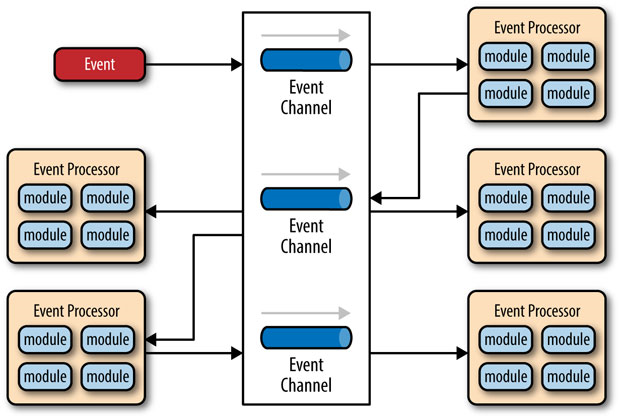
\includegraphics[width=\textwidth]{immagini/ST/schemaevent-driven.png}
					\caption{Diagramma del Design Pattern Event-driven}
				\end{figure}
            \begin{itemize}
				\item \textbf{Scopo:}
					Produrre applicazioni molto scalabili e processare eventi asincroni disaccoppiati.
                \item \textbf{Motivazione:} Gestire le richieste che vengono volte all' applicativo tramite eventi processati in modo asincrono.
                \item \textbf{Applicabilità:}
                	Gestione di eventi attraverso l'utilizzo di elaboratori di eventi e canali per passare gli eventi.		
			\end{itemize}
	
				
	\subsubsection{Singleton}
				\begin{figure}[H]
					\centering
					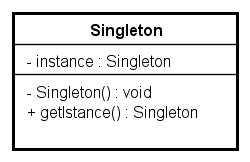
\includegraphics[width=\textwidth]{immagini/ST/schemaSingleton.png}
					\caption{Diagramma del Design Pattern Command}
				\end{figure}
		\begin{itemize}
			\item \textbf{Scopo:} Assicurare che una classe abbia una sola istanza con un unico punto di accesso globale.
			\item \textbf{Motivazione:} È necessario assicurare che esista una sola istanza di alcune classi. Una classe Singleton ha la responsabilità sulle proprie istanze, in modo che nessuna altra istanza possa essere creata, e fornisce un punto di accesso unico.
			\item \textbf{Applicabilità:}
			\begin{itemize}
				\item Deve esistere una ed una sola istanza di una classe in tutta l'applicazione, accessibile dai client in modo noto.
				\item L'istanza deve essere estendibile con ereditarietà, consentendo ai client di non modificare il proprio codice.
			\end{itemize}
		\end{itemize}
	
	\cleardoublepage
	\addcontentsline{toc}{section}{\listfigurename}
	\listoffigures
	
	\cleardoublepage
	\addcontentsline{toc}{section}{\listtablename}
	\listoftables
		
\end{document}